%%
%% This is file `sample-sigconf-authordraft.tex',
%% generated with the docstrip utility.
%%
%% The original source files were:
%%
%% samples.dtx  (with options: `all,proceedings,bibtex,authordraft')
%% 
%% IMPORTANT NOTICE:
%% 
%% For the copyright see the source file.
%% 
%% Any modified versions of this file must be renamed
%% with new filenames distinct from sample-sigconf-authordraft.tex.
%% 
%% For distribution of the original source see the terms
%% for copying and modification in the file samples.dtx.
%% 
%% This generated file may be distributed as long as the
%% original source files, as listed above, are part of the
%% same distribution. (The sources need not necessarily be
%% in the same archive or directory.)
%%
%%
%% Commands for TeXCount
%TC:macro \cite [option:text,text]
%TC:macro \citep [option:text,text]
%TC:macro \citet [option:text,text]
%TC:envir table 0 1
%TC:envir table* 0 1
%TC:envir tabular [ignore] word
%TC:envir displaymath 0 word
%TC:envir math 0 word
%TC:envir comment 0 0
%%
%% The first command in your LaTeX source must be the \documentclass
%% command.
%%
%% For submission and review of your manuscript please change the
%% command to \documentclass[manuscript, screen, review]{acmart}.
%%
%% When submitting camera ready or to TAPS, please change the command
%% to \documentclass[sigconf]{acmart} or whichever template is required
%% for your publication.
%%
%%
\documentclass[sigplan, nonacm]{acmart}
\usepackage{underscore}




%% \BibTeX command to typeset BibTeX logo in the docs

\usepackage{algorithm}
\usepackage{algpseudocode}
\usepackage{amsmath}
\usepackage{makecell}
\usepackage{subcaption}
\usepackage{tikz}
\usepackage{xcolor}
\definecolor{codebg}{HTML}{F7F7F7}
\definecolor{commhop}{RGB}{36,140,64}
\definecolor{commtree}{RGB}{20,150,165}
\definecolor{commfact}{RGB}{210,140,40}
\newsavebox{\codepanelbox}
\newenvironment{codepanel}{%
  \begin{lrbox}{\codepanelbox}%
  \begin{minipage}{\dimexpr\linewidth-8pt\relax}%
}{%
  \end{minipage}%
  \end{lrbox}%
  \setlength{\fboxsep}{4pt}%
  \colorbox{codebg}{\usebox{\codepanelbox}}%
}
\usetikzlibrary{arrows.meta, positioning, calc}
\AtBeginDocument{%
  \providecommand\BibTeX{{%
    Bib\TeX}}}
\newcommand{\at}[2]{(#1)_{#2}}   % \at{i,j,k}{A}  ->  (i,j,k)_{A}
%% Rights management information.  This information is sent to you
%% when you complete the rights form.  These commands have SAMPLE
%% values in them; it is your responsibility as an author to replace
%% the commands and values with those provided to you when you
%% complete the rights form.

%% These commands are for a PROCEEDINGS abstract or paper.

%%
%%  Uncomment \acmBooktitle if the title of the proceedings is different
%%  from ``Proceedings of ...''!
%%
%%\acmBooktitle{Woodstock '18: ACM Symposium on Neural Gaze Detection,
%%  June 03--05, 2018, Woodstock, NY}



%%
%% Submission ID.
%% Use this when submitting an article to a sponsored event. You'll
%% receive a unique submission ID from the organizers
%% of the event, and this ID should be used as the parameter to this command.
%%\acmSubmissionID{123-A56-BU3}

%%
%% For managing citations, it is recommended to use bibliography
%% files in BibTeX format.
%%
%% You can then either use BibTeX with the ACM-Reference-Format style,
%% or BibLaTeX with the acmnumeric or acmauthoryear sytles, that include
%% support for advanced citation of software artefact from the
%% biblatex-software package, also separately available on CTAN.
%%
%% Look at the sample-*-biblatex.tex files for templates showcasing
%% the biblatex styles.
%%

%%
%% The majority of ACM publications use numbered citations and
%% references.  The command \citestyle{authoryear} switches to the
%% "author year" style.
%%
%% If you are preparing content for an event
%% sponsored by ACM SIGGRAPH, you must use the "author year" style of
%% citations and references.
%% Uncommenting
%% the next command will enable that style.
%%\citestyle{acmauthoryear}


%% Relax LaTeX's (conservative) float placement so a wide double-column
%% listing can share a page top with its surrounding text rather than being
%% deferred to a later page.
\renewcommand{\topfraction}{0.9}
\renewcommand{\dbltopfraction}{0.9}
\renewcommand{\bottomfraction}{0.9}
\renewcommand{\textfraction}{0.07}
\renewcommand{\floatpagefraction}{0.7}
\renewcommand{\dblfloatpagefraction}{0.7}
\setcounter{topnumber}{3}
\setcounter{dbltopnumber}{3}
\setcounter{totalnumber}{5}

%%
%% end of the preamble, start of the body of the document source.
\begin{document}

%%
%% The "title" command has an optional parameter,
%% allowing the author to define a "short title" to be used in page headers.
\title{Cyclotron: A Recurrence Language for Expressing Interprocessor Communication}

%%
%% The "author" command and its associated commands are used to define
%% the authors and their affiliations.
%% Of note is the shared affiliation of the first two authors, and the
%% "authornote" and "authornotemark" commands
%% used to denote shared contribution to the research.
%% --- Author list commented out for anonymous ASPLOS submission ---
 \author{Shiv Sundram}
 \email{shiv1@stanford.edu}
 \affiliation{%
   \institution{Stanford University}
   \city{Stanford}
   \state{California}
   \country{USA}
 }

 \author{Akhilesh Balasingam}
 \email{avb03@stanford.edu}
 \affiliation{%
   \institution{Stanford University}
   \city{Stanford}
   \state{California}
   \country{USA}
 }

 \author{Nathan Zhang}
 \email{stanfurd@stanford.edu}
 \affiliation{%
   \institution{Stanford University}
   \city{Stanford}
   \state{California}
   \country{USA}
 }

 \author{Kunle Olukotun}
 \email{kunle@stanford.edu}
 \affiliation{%
   \institution{Stanford University}
   \city{Stanford}
   \state{California}
   \country{USA}
 }

 \author{Fredrik Kjolstad}
 \email{kjolstad@stanford.edu}
 \affiliation{%
   \institution{Stanford University}
   \city{Stanford}
   \state{California}
   \country{USA}
 }

%\author{Anonymous Author(s)}

%%
%% By default, the full list of authors will be used in the page
%% headers. Often, this list is too long, and will overlap
%% other information printed in the page headers. This command allows
%% the author to define a more concise list
%% of authors' names for this purpose.
\renewcommand{\shortauthors}{Anonymous}


%%
%% The abstract is a short summary of the work to be presented in the
%% article.
\begin{abstract}
We present Cyclotron, a compiler that expresses streaming dataflow algorithms
using recurrence equations, which are then compiled to distributed topologies
of interlinked processors. Our compiler lowers a language of recurrences over logical
iteration spaces into per-processor programs of sends, receives,
and computations. In these recurrences, data accesses are not limited to external accesses to memory; data can live separately on the iteration space itself, allowing internal points to  communicate values directly with other points. Users specify this communication directly in the  recurrence language, which allows them to express various communication patterns such as  a nearest-neighbor systolic exchange, a one-to-all broadcast, a bidirectional split ring, or an asymmetric and piecewise broadcast pattern, which are often not supported by standard distributed linear algebra libraries. These recurrences describe the algorithm and communication independently of how they map onto the hardware. A programmer then chooses which dimensions execute across processors and which execute over time, without rewriting the entire program. Users only specify data dependencies across the iteration space, and the compiler safely generates a program, per process, with correct placement of both communication and computational operators according to the chosen space--time mapping. We evaluate distributed matrix multiplication, TRSM, Cholesky, and fused Cholesky--TRSM on up to 16 CPU nodes and 16 GPUs, comparing against ScaLAPACK, SLATE, and cuSolverMp. Cyclotron is competitive with and often outperforms these hand-optimized libraries; for Cholesky, the best communication strategy changes with problem size and architecture.
\end{abstract}

%This expressiveness distinguishesCyclotron from polyhedral and systolic-synthesis frameworks, which uniformizeall communication into nearest-neighbor halo shifts.
%The compiler absorbs the burden of synchronization, automatically ordering sends and receives to guarantee deadlock-free execution on each compilation target.
  %We demonstrate the portability of our approach by compiling to three backends: a distributed-memory CPU cluster, a distributed-memory GPU cluster, and a reconfigurable simulator of systolic arrays and chiplet-style distributed hardware. The recurrences express matrix multiplication (Cannon, SUMMA, PUMMA, weight stationary), prefix sum, Flash Attention, and solvers (triangular solve and Cholesky), and we demonstrate that the compiler can naturally fuse kernels.
%%
%% The code below is generated by the tool at http://dl.acm.org/ccs.cfm.
%% Please copy and paste the code instead of the example below.
%%
\begin{CCSXML}
<ccs2012>
 <concept>
  <concept_id>00000000.0000000.0000000</concept_id>
  <concept_desc>Do Not Use This Code, Generate the Correct Terms for Your Paper</concept_desc>
  <concept_significance>500</concept_significance>
 </concept>
 <concept>
  <concept_id>00000000.00000000.00000000</concept_id>
  <concept_desc>Do Not Use This Code, Generate the Correct Terms for Your Paper</concept_desc>
  <concept_significance>300</concept_significance>
 </concept>
 <concept>
  <concept_id>00000000.00000000.00000000</concept_id>
  <concept_desc>Do Not Use This Code, Generate the Correct Terms for Your Paper</concept_desc>
  <concept_significance>100</concept_significance>
 </concept>
 <concept>
  <concept_id>00000000.00000000.00000000</concept_id>
  <concept_desc>Do Not Use This Code, Generate the Correct Terms for Your Paper</concept_desc>
  <concept_significance>100</concept_significance>
 </concept>
</ccs2012>
\end{CCSXML}



%%
%% Keywords. The author(s) should pick words that accurately describe
%% the work being presented. Separate the keywords with commas.
%\keywords{Do, Not, Use, This, Code, Put, the, Correct, Terms, for,
%  Your, Paper}
%% A "teaser" image appears between the author and affiliation
%% information and the body of the document, and typically spans the
%% page.


\received{2 June 2026}


%%
%% This command processes the author and affiliation and title
%% information and builds the first part of the formatted document.
\maketitle

\section{Introduction}
\label{sec:intro}

Generations of architectural improvements have widened the gap between the cost
of data movement and the cost of computation. Performance optimization is now
dominated by minimizing memory traffic and network communication on distributed architectures. %Whether the target is a cluster of CPUs or heterogeneous processors, distributed machines share a common motif of interconnected processing elements (PEs) wired together via an interconnect topology. 
Extracting performance from such hardware is largely a matter of orchestrating how data
moves through that fabric: laterally between PEs, and temporally as values are
retained in fast memory across steps.

Yet the dominant abstractions for programming these machines do not represent data
movement beyond memory loads/stores. In tensor algebra notation, loop-based IRs, and polyhedral representations, every
data access is a tensor access---logical reads from or writes to memory
locations. Such a program says \emph{what} value each statement consumes, but
not \emph{how} or \emph{where} that value travels between processors or across
time. The movement is left implicit, to be recovered by dependence analysis and
then realized by a lowering pass.

In computational problems where communication is a primary bottleneck, such as in distributed linear algebra (e.g., matrix multiplication), tensor algebra, and recurrences, the best communication policy can vary with input size, tile size, interconnect, and processor architecture. Yet standard distributed libraries like ScaLAPACK \citep{choi1992scalapack} or SLATE \citep{gates2019slate} either hard-code communication policies or expose only a small set of predefined options. Consequently, the best communication schedule for a particular problem and architecture may not be available to the programmer.



Compiler frameworks avoid pitfalls of writing distributed code by hand, which is error-prone and can lead to indefinite hangs from mismatched or incorrectly ordered communication, while also being difficult to optimize (e.g., overlapping communication with computation).
Polyhedral frameworks have made important steps forward in modeling relationships between iteration spaces and memory accesses. Existing polyhedral frameworks, like AutoSA \citep{autosa} for systolic-array synthesis and AlphaZ for distributed-memory code generation,\cite{alphaz} lower dependencies into nearest-neighbor transfers; both therefore effectively commit to a systolic realization of communication. As a result, alternative realizations of the same logical dependence, such as a one-to-all broadcast, a tree-broadcast, or heterogeneous combinations of broadcast and forwarding, are not supported.

This limitation stems from what the user program leaves unspecified. With polyhedral frameworks, users write equations or loops over array accesses, and the compiler analyses the program to identify where communication should occur. There are typically many ways  to realize data movement, but without user input the compiler must choose among them. For example, AutoSA and AlphaZ only generate code where communication is limited to between neighboring PEs. This can leave performance on the table when a different communication strategy better matches the problem size or target architecture. Stellar \citep{genc2024stellar}, a framework for spatial accelerator design, allows users to specify dataflow and lets iteration-space points receive data from neighbors, supporting systolic patterns, but does not generalize beyond them.


This paper presents the Cyclotron compiler that makes the communication schedule
a first-class part of the input program. The program can express many different communication patterns as recurrence equations. These include systolic exchanges, one-to-all broadcast, tree-broadcast, bidirectional split rings, or asymmetric, piecewise combination of communication policies, in which different subdomains of a program and processor grid carry different communication policies. A user can specify that a data tile travel via nearest-neighbor hops in one part of the processor grid, via a tree broadcast in other parts, and bidirectionally in another.

\begin{figure}[t]
\centering
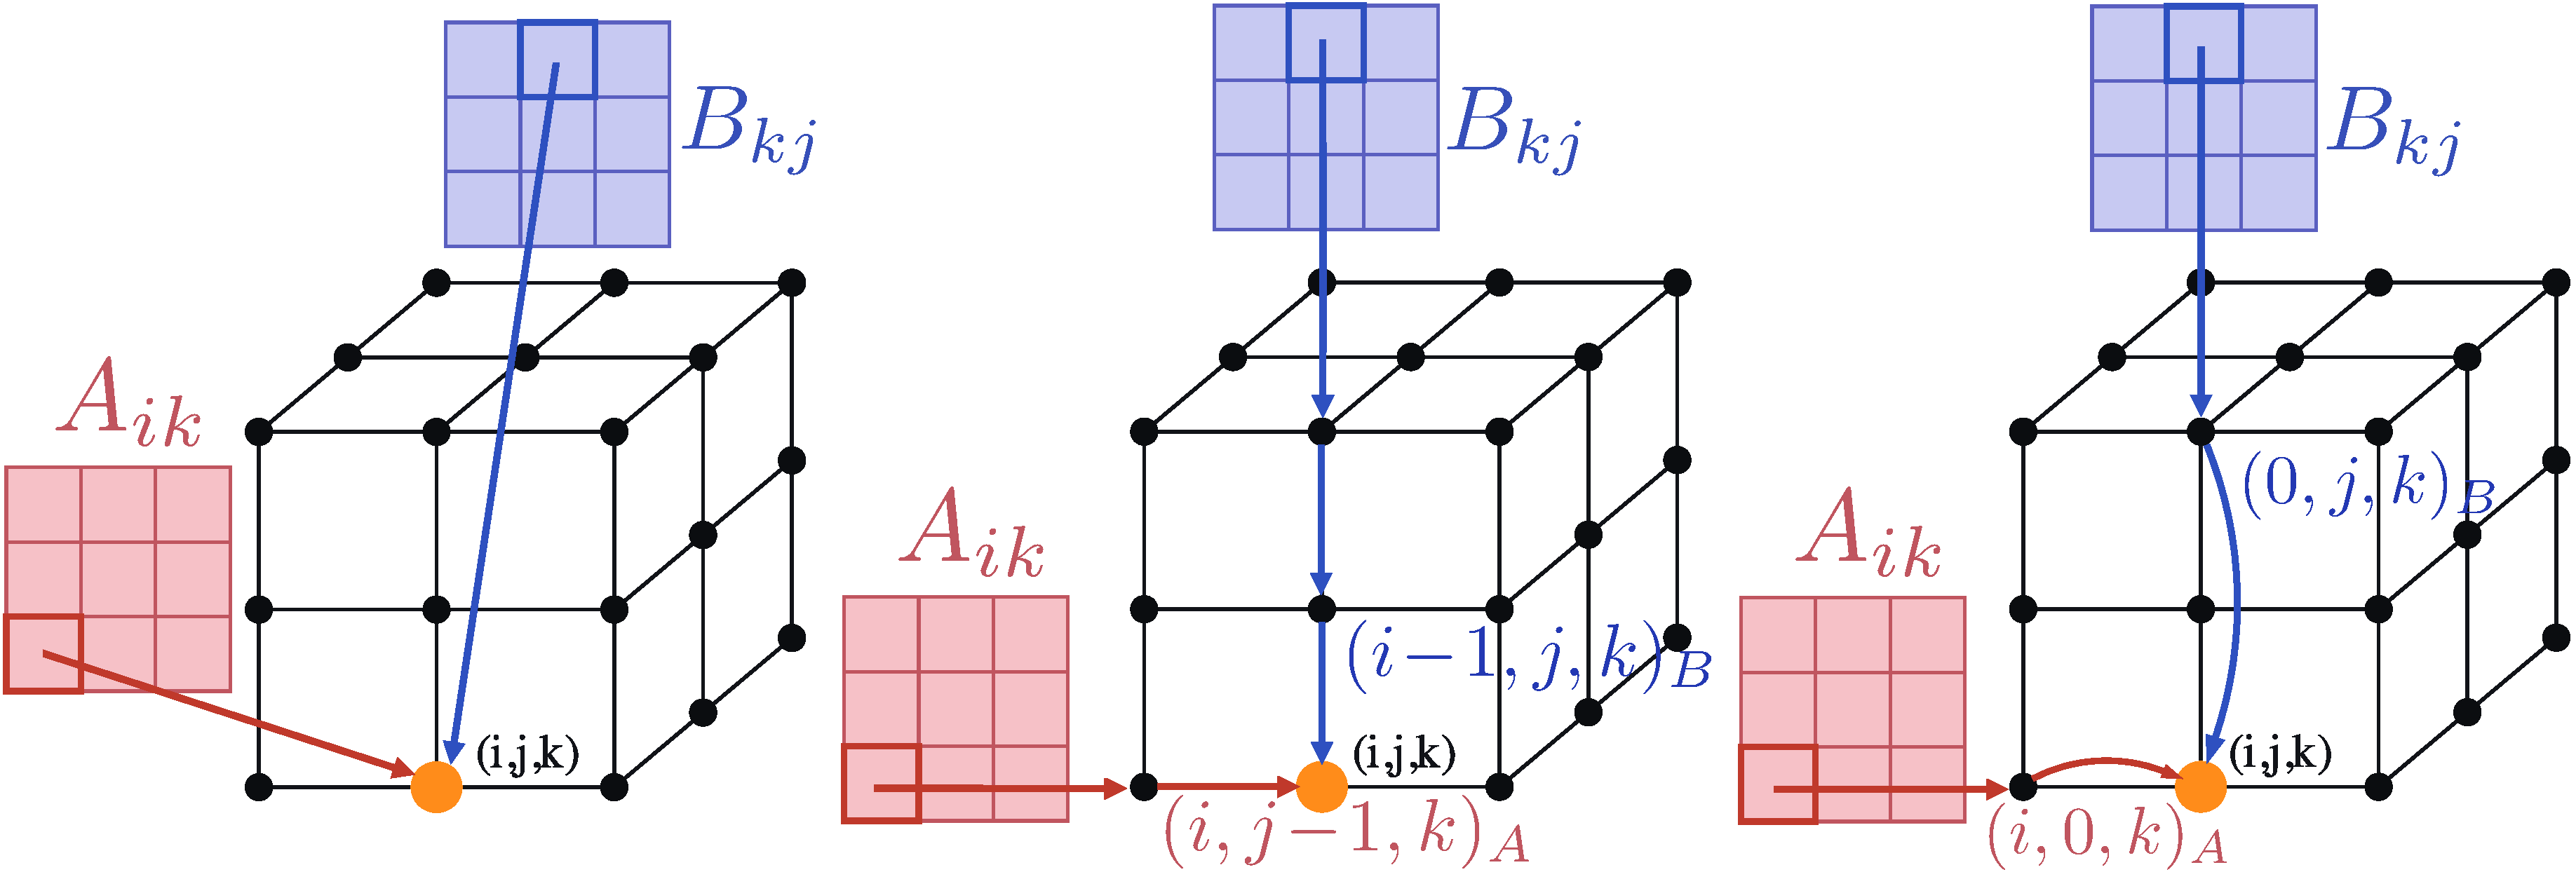
\includegraphics[width=\linewidth]{memvspace3.pdf}
\caption{Three spatial matrix multiplies. Left: each point reads operands
$A_{ik}$ and $B_{kj}$ directly from memory. Middle: each operand is loaded once
at a boundary face, and interior points receive $A$ and $B$ systolically
from neighbors. Right: each point receives its data directly from boundaries.
}
\label{fig:memory-vs-space-intro}
\end{figure}
In Cyclotron, the programmer writes
computation as a system of recurrences that can index into tensors that live on the iteration space in addition to tensors that live in memory, thus controlling data movement. Figure~\ref{fig:memory-vs-space-intro} illustrates the 3D iteration space of a matrix multiply, contrasting a program where data is accessed exclusively from tensors with two different programs where data is also obtained from points in the iteration space. What differs is how each value is obtained: directly from the tensor, from a neighboring iteration-space point, or from a boundary point via broadcasts. In Cyclotron, a value on the iteration space is named not only by which tensor element it is (e.g., $A_{ij}$) but by the point in the iteration space at which it lives, written
$(i,j,k)_{A}$. Movement, like the systolic transfer $(i,j,k)_A \leftarrow (i,j\!-\!1,k)_A$, is expressed in the same coordinate system as computation: a recurrence relating a value at one point to another point \emph{is} a data movement. A separate per-dimension annotation declares whether each dimension is spatial (movement between PEs) or temporal (retention across steps). Data movement is not limited to nearest neighbors, and because the recurrence is written independently of this annotation, the same program can be used to generate different spatial mappings.

The user's input recurrences are unordered. The ordering of compute and communication operations depends on which dimensions are mapped in space and time. Cyclotron's dependency algorithm uses this mapping to derive correct orderings, relieving users of the need to manually sequence such operations and avoiding indefinite waits caused by incorrect communication ordering.

These recurrences are compiled to distributed code through a fixed pipeline: a space--time mapping folds the iteration space and inserts a temporal loop. Our dependency-management algorithm resolves data dependencies into coupled sends and receives. Synchronization-aware control flow is inserted according to the target protocol. A final pass can apply a block-cyclic decomposition and deduplicate communication. %The resulting code is then executed on the target backend by a target-specific runtime.


Cyclotron lets programmers explore communication strategies with minimal program changes. The resulting code is competitive with, and often outperforms, expert-tuned libraries. We make the following contributions:
\begin{itemize}
  \item A recurrence-based programming model where communication is a first-class programmable concern, separate from computation and space--time mapping, enabling programmers to express and compose systolic, broadcast, ring, tree, and heterogeneous piecewise communication strategies.
%(§\ref{sec:notation}).
  \item A dependency-management algorithm that uses the chosen space--time mapping to order computation and communication from unordered recurrences
  %(§\ref{sec:compilation}).
  \item A complete compilation pipeline integrating the dependency algorithm with transformations that handle synchronization, block-cyclic decomposition and communication deduplication, generating efficient distributed programs.
\end{itemize}

By exploring different communication schedules, 
we demonstrate $1.7$--$1.8\times$ over ScaLAPACK for matrix multiply.
For Cholesky on up to 16 CPU nodes, we observe  $1.34$--$1.68\times$  speedup over ScaLAPACK  on CPUs
and $1.01-1.24 \times$ speedup over SLATE on GPUs (which uses CPU-side communication), and 1.12--1.28$\times$ speedup over cuSolverMp, Nvidia's optimized multi-GPU vendor library, when only using direct GPU-GPU communication. We demonstrate benefits of simultaneously composing different space--time mappings and how Cyclotron natively fuses kernels.


\section{Motivating Example}
\label{sec:motivation}
\label{sec:cholesky}

\begin{figure}[t]
\centering
\begin{minipage}[t]{0.49\linewidth}
\vspace*{0pt}
% --- kij (RIGHT-LOOKING) ---
\begin{subfigure}[t]{\linewidth}
\centering
\scriptsize
\begin{codepanel}
\begin{algorithmic}
\For{$k = 0$ \textbf{to} $N{-}1$}
    \State $\text{POTRF}(L_{k,k})$
    \For{$i = k{+}1$ \textbf{to} $N{-}1$}
        \State $\text{TRSM}(L_{i,k}, L_{k,k})$
    \EndFor
    \For{$i = k{+}1$ \textbf{to} $N{-}1$}
        \State $\text{SYRK}(L_{i,i}, L_{i,k})$
        \For{$j = k{+}1$ \textbf{to} $i{-}1$}
            \State $\text{GEMM}(L_{i,j}, L_{i,k}, L_{j,k})$
        \EndFor
    \EndFor
\EndFor
\end{algorithmic}
\end{codepanel}
\caption{Right-looking $kij$.}
\label{fig:chol-kij}
\end{subfigure}

\vspace{0.6em}

% --- ijk (UP-LOOKING INNER PRODUCT) ---
\begin{subfigure}[t]{\linewidth}
\centering
\scriptsize
\begin{codepanel}
\begin{algorithmic}
\For{$i = 0$ \textbf{to} $N{-}1$}
    \For{$j = 0$ \textbf{to} $i{-}1$}
        \For{$k = 0$ \textbf{to} $j{-}1$}
            \State $\text{GEMM}(L_{i,j}, L_{i,k}, L_{j,k})$
        \EndFor
        \State $\text{SYRK}(L_{i,i}, L_{i,j})$
        \State $\text{TRSM}(L_{i,j}, L_{j,j})$
    \EndFor
    \State $\text{POTRF}(L_{i,i})$
\EndFor
\end{algorithmic}
\end{codepanel}
\caption{Up-looking $ijk$.}
\label{fig:chol-ijk}
\end{subfigure}
\end{minipage}\hfill
\begin{minipage}[t]{0.49\linewidth}
\vspace*{0pt}
% --- ijk + communication (systolic panels, broadcast Lc) ---
\begin{subfigure}[t]{\linewidth}
\centering
\scriptsize
\begin{codepanel}
\begin{algorithmic}
\State $i,j \leftarrow \text{rank}()$
\For{$k = 0$ \textbf{to} $j$}
    \If{$k < j$}
        \State $\text{Recv } L_{i,k}\text{: }(i,\, j{-}1)$
        \State $\text{Send } L_{i,k}\text{: }(i,\, j{+}1)$
        \If{$i > j$}
            \State $\text{Recv } L_{j,k}\text{: }(i{-}1,\, j)$
            \State $\text{GEMM}(L_{i,j}, L_{i,k}, L_{j,k})$
        \Else
            \State $L_{j,k} \leftarrow L_{i,k}$
            \State $\text{SYRK}(L_{i,i}, L_{j,k})$
        \EndIf
        \State $\text{Send } L_{j,k}\text{: }(i{+}1,\, j)$
    \EndIf
    \If{$k = j,\ i > j$}
        \State $\text{Recv } L_{j,j}\text{: }(j,j)$
        \State $\text{TRSM}(L_{i,j}, L_{j,j})$
        \For{$d = 1$ \textbf{to} $N{-}j{-}1$}
            \State $\text{Send } L_{i,j}\text{: }(i,\, j{+}d)$
        \EndFor
    \EndIf
    \If{$k = j = i$}
        \State $\text{POTRF}(L_{i,i})$
        \For{$d = 1$ \textbf{to} $N{-}i{-}1$}
            \State $\text{Send } L_{i,i}\text{: }(i{+}d,\, i)$
        \EndFor
    \EndIf
\EndFor
\end{algorithmic}
\end{codepanel}
\caption{Per-processor lowering of $ijk$.}
\label{fig:chol-lowering}
\end{subfigure}
\end{minipage}

\caption{Two Cholesky loop nests (a,b) and a distributed lowering of the
up-looking nest (c). The order of the compute statements differs between the
two sequential variants, as do the number of inner loops and tensor indexing. The 
distributed nest (c) adds send/recv statements. $\text{Recv}\,X\text{:}\,(r,c)$/$\text{Send}\,X\text{:}\,(r,c)$ name
the peer.}
\label{tab:cholesky_variants}
\end{figure}

\begin{figure}[t]
\centering
\small
\begin{subfigure}[t]{\linewidth}
\centering
\begin{codepanel}
\begin{minipage}{\linewidth}
\raggedright
\noindent
\(\displaystyle
\begin{aligned}
\text{default\_constraint}
&= ((i, j, k),\; i > j > k) \\[0.25em]
(i, i, 0)_{Ls} &\leftarrow A_{ii},
\qquad
(i, j, 0)_{Lg} \leftarrow A_{ij} \\[0.2em]
(i, j, j)_{Lgl}
&\leftarrow \text{TRSM}\big(
  (i, j, j)_{Lc},\;
  (i, j, j)_{Lg}
\big) \\[0.15em]
\color{commhop}
(i, j, k)_{Lgl}
&\leftarrow (i, k, k)_{Lgl}
\qquad (i \ge j) \\[0.15em]
\color{black}
(i, i, k)_{Lgu}
&\leftarrow (i, i, k)_{Lgl} \\[0.15em]
\color{commtree}
(i, j, k)_{Lgu}
&\leftarrow (i - 1, j, k)_{Lgu} \\[0.15em]
\color{black}
(i, j, k)_{Lg}
&\leftarrow \text{GEMM}\big(
  (i, j, k)_{Lgl},\;
  (i, j, k)_{Lgu}, \\
&\qquad\quad
  (i, j, k - 1)_{Lg}
\big) \\[0.15em]
(i, i, k)_{Ls}
&\leftarrow \text{SYRK}\big(
  (i, i, k)_{Lgu},\;
  (i, i, k - 1)_{Ls}
\big) \\[0.15em]
(j, j, j)_{Lc}
&\leftarrow \text{POTRF}\big(
  (j, j, j - 1)_{Ls}
\big) \\[0.15em]
\color{commfact}
(i, j, j)_{Lc}
&\leftarrow (j, j, j)_{Lc}
\end{aligned}
\)
\end{minipage}
\end{codepanel}
\caption{Broadcast $L_{gl}$/$L_c$, systolic $L_{gu}$ (matches Figure~\ref{fig:chol-lowering}).}
\label{fig:chol-dataflow-bcast}
\end{subfigure}

\vspace{0.45em}

\begin{subfigure}[t]{\linewidth}
\centering
\scriptsize
\begin{codepanel}
\begin{minipage}{\linewidth}
\raggedright
\noindent
\(\displaystyle
\begin{aligned}
\color{commhop}
(i, k{+}m, k)_{Lgl}
&= (i, k, k)_{Lgl}
\quad m\in\{1,2,3\}
&& \text{(anchored hops)} \\[0.2em]
\color{commhop}
(i, j, k)_{Lgl}
&= (i, j{-}1, k)_{Lgl}
\quad (j > k{+}3)
&& \text{(relay)} \\[0.2em]
\color{commtree}
(i, j, k)_{Lgu}
&= (i{-}s, j, k)_{Lgu}
\quad (j{+}s \le i < j{+}2s)
&& \text{(tree, } s\in\{1,2,4\}) \\[0.2em]
\color{commfact}
(i, j, j)_{Lc}
&= (i{-}s, j, j)_{Lc}
\quad (j{+}s \le i < j{+}2s)
&& \text{(tree, } s\in\{1,2,4\})
\end{aligned}
\)
\end{minipage}
\end{codepanel}
\caption{Same compute; only communication modified}
\label{fig:chol-dataflow-alt}
\end{subfigure}

\caption{One Cholesky dataflow in Cyclotron, devoid of the statement
ordering, inner-loop nesting, and re-indexing required across the variants
in Figure~\ref{tab:cholesky_variants}. Panel~(a) is the broadcast/systolic
spelling: with $i$ and $j$ spatial and $k$ temporal it lowers to
Figure~\ref{fig:chol-lowering}. Panel~(b) keeps every compute recurrence
and rewrites only $L_{gl}$, $L_{gu}$, and $L_c$---a depth-3 modified ring
along the row and doubling trees down the column.}
\label{fig:tensor_constraints}
\end{figure}

We use distributed, blocked Cholesky decomposition as a motivating example.
Cholesky factors a symmetric positive-definite matrix into a triangular factor and its transpose.
 In a blocked implementation, processors operate on matrix tiles using four dense BLAS/LAPACK kernels:
  POTRF, TRSM, SYRK, and GEMM. Different processors execute different sequences of these operations 
  depending on their position in the processor grid and the current step of the factorization.
  Moreover, these operations depend on values produced elsewhere in the grid, and
  those dependences can be realized using different communication strategies; 
  communication is not simply a uniform pattern of nearest-neighbor shifts. The computation is load--imbalanced, in which critical paths occurring in certain portions of the grid asymmetrically affect work on downstream processors.

Figure~\ref{tab:cholesky_variants} shows two loop-based formulations of blocked Cholesky. 
Even in the serial, non-distributed case, the loop form is coupled to the dependencies among the four kernels. In other words, changing the loop ordering requires more than merely permuting loop headers, as one can for perfectly nested computation such as matrix multiplication. 
It changes loop bounds, the number and placement of inner loops, the ordering of kernel calls, 
and their indexing. In loop--based spatial frameworks, loop dimensions/nesting--order are also used to determine
which parts of the computation execute across processors and which execute over time. 
Changing the space--time mapping can therefore require restructuring the program rather than
simply changing a mapping decision.

Distributing the computation makes the control flow more complex (Figure~\ref{fig:chol-lowering}). The programmer must place sends and receives, add processor- and time-dependent branches,
 construct fan-out send loops, and ensure that every receive has a matching send. 
 Incorrect send/receive pairing can result in indefinite hangs. Changing the communication strategy may require restructuring 
 this control flow even though the underlying computation is unchanged.

Cyclotron instead separates these concerns. The computation is written once in a loopless recurrence form. Figure~\ref{fig:tensor_constraints} shows a Cyclotron recurrence specification of a Cholesky decomposition. It generates the exact code corresponding to Figure~\ref{fig:chol-lowering}, 
while the space--time mapping is specified separately. 
Computation and communication are both expressed as recurrences over iteration-space points, 
so changing the communication strategy  (e.g., from systolic forwarding to broadcast or a tree) changes
only the communication recurrences, not the computation. Figure ~\ref{fig:chol-dataflow-alt} 
shows the same communication recurrences rewritten with a different communication strategy. The communication
of $L_{gu}$ and $L_{c}$ now uses hierarchical doubling tree-broadcasts. 
The communication of $L_{gl}$ is now a modified increasing ring, where it initially broadcasts
to the three nearest neighbors to its right, with the third neighbor and the remaining neighbors
communicating systolically. In the equivalent per-processor imperative program, 
this four-line change more than doubles the code size of the program in Figure~\ref{fig:chol-lowering},
because separate control flow is required for the modified ring (a hybrid systolic-broadcast strategy) and for the doubling tree.

Finally, these recurrence specifications are unordered. Given a space--time mapping and target communication protocol, 
Cyclotron's dependency-management algorithm determines a valid ordering of computation, 
sends, and receives.



\definecolor{codebg}{gray}{0.96}
\section{Notation}
\label{sec:notation}



Recurrences and tensor algebra have traditionally been defined over indexed
tensors \citep{recuma, reptile, vinaithirthan2026compiling, kjolstad2017taco}. Cyclotron augments this with recurrences over \emph{iteration spaces}.
In conventional recurrence and tensor-algebra equations, each tensor
access ($A_{ij}$, or \texttt{A[i][j]}) denotes a logical access to a memory
hierarchy. This model maps well to von Neumann programs on a
single processor, but lacks any mechanism for describing data
that propagates through time or across processors as every data reference is a
tensor access.

Cyclotron's notation describes both computation and communication. First,
\emph{computations} are defined as recurrences over an iteration space
(Section \ref{sec:recurrences}). This way, data may live on the iteration space itself, in addition to living in external tensors. Second, \emph{communication patterns} are specified
in that same language (Section \ref{sec:communication}), as a transfer between two points in the iteration space: a systolic relay, a
broadcast, or a piecewise hybrid of the two is just another recurrence,
distinguished only by the shape of its coordinate expressions. Figure ~\ref{fig:memory-vs-space-intro} illustrates this dichotomy of accessing data from memory versus the iteration space.

\subsection{Defining Recurrences over Iteration Spaces}
\label{sec:recurrences}

\newcommand{\bnfdef}{\mathrel{::=}}
\newcommand{\bnfalt}{\mathrel{\mid}}
\begin{figure}[t]
\centering
\small
\[
\begin{array}{rlcl}
    \multicolumn{4}{l}{\textsf{ConstInt}~n \quad \textsf{Tensor}~t \quad \textsf{IndexVar}~v} \\
    \textsf{Index}        & i  & \bnfdef & v \bnfalt n \bnfalt v+n \\
    \textsf{TensorAccess} & ta & \bnfdef & t_{i_1,\ldots,i_d} \\
    \textsf{IterAccess}   & ia & \bnfdef & (i_1,\ldots,i_d)_t \\
    \textsf{Expr}         & e  & \bnfdef & ta \bnfalt ia \bnfalt \textit{const} \bnfalt \operatorname{func}(e_1,\ldots,e_n) \\
                          &    &         & \bnfalt e+e \bnfalt e\,e \bnfalt \cdots \\
    \textsf{Recurrence}   & r  & \bnfdef & ia \leftarrow e \\
    \textsf{Constraint}   & c  & \bnfdef & i < i \bnfalt i \leq i \bnfalt i = i \bnfalt i \geq i \bnfalt i > i \\
    \textsf{Stmt}         & s  & \bnfdef & r \bnfalt r \;\; c^* \\
    \textsf{Program}      & p  & \bnfdef & s \bnfalt s,p
\end{array}
\]
\caption{Input grammar. \emph{func} does not support recursion.}
\label{fig:grammar}
\end{figure}

In a spatial program, data moves laterally between processors and can be retained
in fast memory across time. If processors are assigned distinct portions of a
program's iteration space, then dataflow across the iteration space corresponds
directly to dataflow between processors, or to dataflow across time.




Cyclotron makes data movement across an iteration space expressible by allowing tensors to be stored on the iteration space, in addition to in memory. Figure~\ref{fig:grammar} shows Cyclotron's grammar. Given a three-tensor $A$
that lives on a three-dimensional iteration space $(i,j,k)$, we write$(i,j,k)_{A}$ to denote the value/tile of $A$ at point $(i,j,k)$ of the iteration space. Figure~\ref{fig:cannonIR} uses this notation to give the
complete dataflow of a systolic matrix multiply in six lines. Movement is encoded by coordinate differences. For example, $(i,j,k)_A \leftarrow (i,\,j{-}1,\,k)_{A}$ propagates the $A$ one step along the second
dimension $j$. This step corresponds to data moving to a neighboring processor if the user declares that dimension to be \emph{spatial}, or to data being retained
on the same processor for the next time step if the user declares the dimension \emph{temporal}. Thus, the same recurrence specification can support different space--time
mappings without changing the equations. In the classical Cannon's algorithm, $i$ and $j$  are spatial and $k$ temporal. This yields systolic movement of $A$ and $B$ and a temporal accumulator for $C$, which is retained in a register from one timestep to another. 

\begin{figure}[t]
\centering
\captionsetup{font=small}
\small

\colorbox{codebg}{%
\begin{minipage}{0.97\columnwidth}
\[
\setlength{\jot}{2pt}
\begin{aligned}
(i,0,k)_{A} &\leftarrow A_{ik}
    && \text{inject $A$} \\
(0,j,k)_{B} &\leftarrow B_{kj}
    && \text{inject $B$} \\
(i,j,0)_{C} &\leftarrow 0
    && \text{init.\ accumulator} \\
(i,j,k)_{A} &\leftarrow (i,j\!-\!1,k)_{A}
    && \text{receive $A$ along $j$} \\
(i,j,k)_{B} &\leftarrow (i\!-\!1,j,k)_{B}
    && \text{receive $B$ along $i$} \\
(i,j,k)_{C} &\leftarrow
    (i,j,k)_{A}(i,j,k)_{B}
    +(i,j,k\!-\!1)_{C}
    && \text{multiply--accum.}
\end{aligned}
\]
\end{minipage}%
}

\caption{Cyclotron specification of a systolic matrix multiplication.}
\label{fig:cannonIR}
\end{figure}

\begin{figure*}[t]
\centering
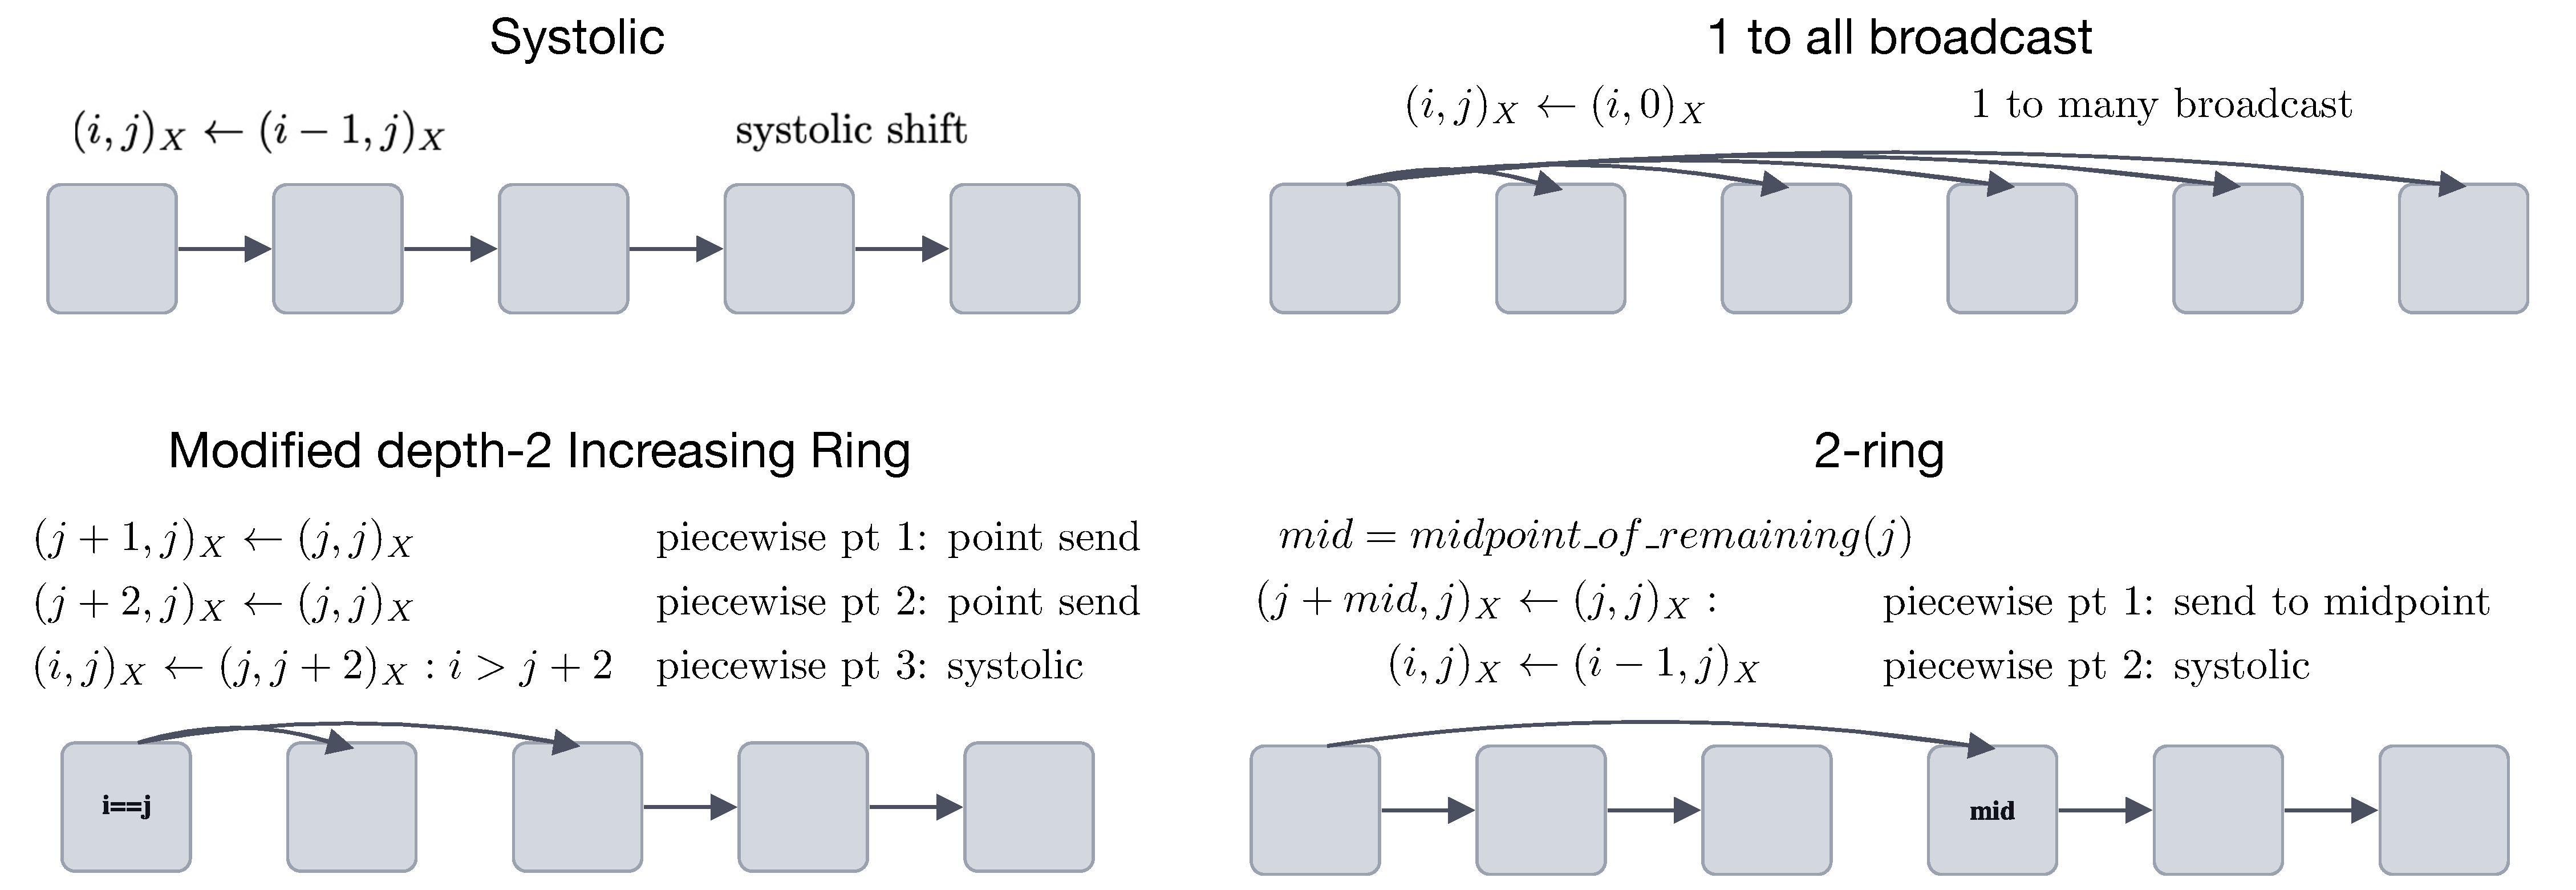
\includegraphics[width=0.92\textwidth]{comm_patterns_pretty7.pdf}
\caption{Four sample expressible Cyclotron communication patterns, defined over $(i,j)$ with $i$ spatial and $j$ temporal.}
\label{fig:comm-patterns}
\end{figure*}


%expressed through the coordinates themselves: a recurrence relates a value at one point to a value at another, and the difference between the two points \emph{is} the movement. Writing an equation that relates $(i,j,k)_{A}$ to

%the $A$ and $B$ recurrences, whose offsets lie along $j$ and $i$, become hops between neighboring processors, while the $C$ recurrence, whose offset lies along $k$, becomes the accumulator each processor retains in a register from one timestep to the next.

%\begin{figure}[t]
%\centering
%\includegraphics[width=\linewidth]{memvspace.pdf}
%\caption{The same interior point $(i,j,k)$ of a matrix multiply %program's iteration space. Left: each point reads its operands
%$A_{ik}$ and $B_{kj}$ directly from memory. Middle: each operand %is loaded once
%at a boundary face---$A$ at $(i,0,k)$, $B$ at $(0,j,k)$---and then %relayed systolically
%through space, so the interior point receives $A$ and $B$
%from its neighbors $(i,j{-}1,k)$ and $(i{-}1,j,k)$ rather than %memory. Right: each point receives its data directly from source %points.
%} 
%\label{fig:memory-vs-space}
%\end{figure}

%Computation on the iteration space is carried out with functions; a function ingests other values living on the iteration space. In Figure~\ref{fig:cannonIR} there is one function, a matrix multiply-accumulation, defined as $(i,j,k)_C = (i,j,k)_A (i,j,k)_B + (i,j,k-1)_C$. The function takes in a tile of $A$ and tile of $B$ living on the current point, multiplies them, and accumulates the result to the tile of $C$ living at neighboring point $(i,j,k-1)$. 

Computation on the iteration space is expressed with functions over iteration-space values. For example, Figure~\ref{fig:cannonIR} defines matrix multiply-accumulate as
$(i,j,k)_C = (i,j,k)_A (i,j,k)_B + (i,j,k-1)_C$. Because movement is carried in the same coordinate system as computation, it is written in the equations rather than recovered by a separate dependence analysis. In loop-based dataflow languages every data access is a tensor access, so the language can detect that a value must be broadcast across the iteration space but has no notion of how or where the data moves; in Cyclotron the movement and the computation it serves are expressed in one grammar.
%The two send lines that close Figure~\ref{fig:cannonIR} (written with $\rightarrow$) are the outbound halves of the two receives, making each stream's path through a processor explicit; §\ref{sec:communication} catalogues the communication patterns this vocabulary expresses, and §\ref{sec:emitting-comm} describes how sends are, in most cases, deduced rather than written.

% NOTE (2026-07-24): two motivation/positioning deep-dives trimmed from here.
% The URE/polyhedral positioning paragraph moved to \section{Related Work};
% the loop-order-coupling argument is already made in §2.2 (sec:cholesky), so
% only its non-redundant core is kept below.
%The notation is loop-free: in the \emph{specification}, the dimensions of the iteration space are unordered, and every index variable is in scope at every
%statement---the loop-order coupling dissected in Section~\ref{sec:cholesky}has nosyntax to be written in. The recurrences in Figure~\ref{fig:cannonIR} carry no
%loop order: nothing in them commits $k$ to be the sequential dimension, and all three index variables are available to every line. Ordering is deferred.

Cyclotron specifications are loop-free and unordered. All iteration-space indices are in scope at every recurrence, and no loop order is imposed. The loop-order coupling dissected in Section~\ref{sec:cholesky} (e.g. the $ijk$ vs $kij$ Cholesky loops) is not relevant with recurrences. A separate space--time map linearizes the dependence relation, while remaining separate from the equations to avoid overspecializing programs and to promote program reuse.

\subsection{Iteration Space Boundaries and Subspaces}
Different operations may be defined on subspaces or partitions of the iteration space. Cyclotron supports this through substitutions, which fix indices to constants or other index variables, and constraints, which specify equalities or inequalities over the indexing variables.

Substitutions describe lower-dimensional subspaces of an iteration space. In Figure~\ref{fig:cannonIR}, matrix-multiply operations (i.e., GEMM) are defined over the full rectangular iteration space $(i,j,k)$, while boundary operations are defined on lower-dimensional faces. For example, $(i,0,k)_{A} \leftarrow A_{ik}$ loads tiles from memory where data enters the iteration space, and $(i,j,0)_{C} \leftarrow 0$ seeds the accumulator on the face $k=0$.

Constraints describe subspaces or partitions of a rectangular iteration space. The Cholesky decomposition's inner iteration space is a 3D triangular pyramid defined by $i>j>k$. Figure~\ref{fig:tensor_constraints} shows that a global default constraint can apply to each recurrence, while individual recurrences may specify their own constraints to override it.


%Constraints (equalities and inequalities) describe either subspaces, or partitions of a rectangular iteration space. The Cholesky decomposition iteration's inner space is a 3D triangular pyramid, where the indexing variables constrain each other via $i>j>k$. Figure ~\ref{fig:tensor_constraints} shows that the user can define a global, default inequality that applies to each recurrence via $\text{default\_constraint} = i>j>k$. They can also associate individual recurrences with their own inequalities, to override the default constraint, like with $(i,j,k)_{Lgl} \leftarrow (i,k,k)_{Lgl} \;\; i \ge j$. Per-recurrence constraints can have the same effect as a substitution: ($(i,j,k)_C \leftarrow 0 \;\; j==0)$ is akin to saying $(i,j,0)_C \leftarrow 0$, but is simply more verbose. 
 

Substitutions may also involve other index variables. Cholesky, for example, defines operations on diagonal subspaces such as \(i=j=k\), which form a 1D subset of the 3D iteration space in Figure~\ref{fig:chol-lowering}. We express these by \emph{gimbal-locking} dimensions: substituting one index variable for another, as in \((j,j,j)\). 
Each index variable has a native dimension. Here \(i\) is the first, \(j\) the second, and \(k\) the third. Substituting an index in a non-native dimension equates the indices and locks the dimensions together. Thus \((i,i,i)\), \((j,j,j)\), and \((k,k,k)\) all denote the same diagonal subspace. This differs from loop-based forms, where the specific diagonal index used, such as \(L_{kk}\) versus \(L_{ii}\),  can depend on the surrounding loop structure.

%Substitutions may involve other index variables, not just constants. Cholesky, for example, defines operations on diagonal subspaces such as \(i=j=k\), which form a 1D subset of the 3D iteration space (e.g., the POTRF operations in Figure~\ref{fig:chol-lowering}). We express these by \emph{gimbal-locking} dimensions: substituting one index variable for another, as in \((j,j,j)\). Each index variable has a native dimension. Here \(i\) is the first, \(j\) the second, and \(k\) the third. Substituting an index in a non-native dimension equates the indices. Equating the indices locks all three dimensions together, forcing them to share one effective index. Thus \((i,i,i)\), \((j,j,j)\), and \((k,k,k)\) denote the same diagonal subspace. This differs from loop-based forms, where the specific diagonal index used, such as \(L_{kk}\) versus \(L_{ii}\),  can depend on the surrounding loop structure.

Substitutions, like per-recurrence constraints, override the default constraint when they conflict. If multiple recurrences match a point, the most specific subspace (the one with the most substitutions) takes precedence. For example, \((0,2,2)\) matches a recurrence defined on \((i,j,j)\) over one defined on \((i,j,k)\). Ties are undefined.


%Substitutions can involve other index variables, not just constants. Like Cannon's, Cholesky defines operations on 2D subspaces, and even 1D spaces. However, some of these subspaces themselves are diagonal, not rectangular. CHOL operations are defined on all points where $i==j==k$, representing a 1D subspace. We can define such subspaces by \emph{gimbal-locking} dimensions, which we define as a substitution of an index variable with another index variable (e.g. $(j,j,j)$). In our programs, each index variable has a native dimension; $i$ defines the first dimension, and $j$ and $k$ the second and third. Equating $j$, which natively defines the second dimension, to $i$ and $k$ locks all three variables together. They all now index the same effective dimension, resulting in a 1D subspace. Users can symmetrically define $(j,j,j)$ as $(i,i,i)$ or $(k,k,k)$, since they mean the same thing.  This unlike the loop forms, where the specific choice of diagonal index ($L_{kk}$ vs $L_{ii}$) matters for correctness; the user must use the iteration variable of the outer most loop. 
%Substitutions, like individual constraints, will override the default constraint if they conflict with it. In other words, the default $(i>j>k)$ defines an inner iteration space, and substitutions like $(j,j,j)$ or $(i,k,k)$ define its boundaries. In cases where a point may belong to multiple defined subspaces, the most specific subspace, or rather the one with the most substitutions, takes priority. At execution time, point $(0,2,2)$ will bind to any expression defined on $(i,j,j)$ over any defined on $(i,j,k)$. An expression specifically defined on $(0,2,2)$ would trump both. Ties are undefined; this is akin to template matching in a type system; the most specific template is the one that binds.

%Such substitutions are akin to the gimbal-locking of Eulerian systems used to define 3D rotations; when two rotational axes line up in parallel, the result is a sudden loss of one degree of freedom. Substitutions and constraints allow us to express  Cholesky decomposition, which is riddled with imperfectly nested statements and control flow, in a clean, loop-free form, free of the peculiarities exhibited by its loop-based counterparts. Furthermore, it allows us to describe programs in an order-free notation; users do not have to think of the dependencies, indexing and the correct ordering of statements demanded by the loop-based forms. 

%For a triangular iteration space---say one whose
%interior is the strict region $k < j < i$---a boundary is instead specified by
%\emph{gimbal-locking}. Because the interior is strict, its bounding faces do not belong
%to the interior itself; gimbal-locking selects a face of the \emph{closure} (i.e., the outer boundary) of that constrained
%the region. The point $(i,\,i,\,k)$ places the index $i$ in the slot normally
%occupied by $j$, forcing $i = j$ in this instance, and thereby denotes the
%two-dimensional face $j = i$ on the closure of $k < j < i$. Reading $(i,i,k)$
%this way is therefore not a contradiction of the strict bound $j < i$: it names
%a boundary face of the closure, not a point of the open interior. Note that
%gimbal-locking plays two roles at once: it \emph{names} an outer boundary face, and by
%collapsing one index onto another it \emph{lowers the dimensionality} of the
%computation on that face, so the same mechanism that identifies the edge also
%gives the reduced-dimension recurrence that runs on it. 

\subsection{Specifying Communication}
\label{sec:communication}


Because movement is written as coordinate offsets, a \emph{communication
pattern} is determined by the recurrence's coordinate expressions:
which coordinates carry offsets, and whether the source point is named
relative to the consumer or absolutely. Figure~\ref{fig:comm-patterns}
illustrates four example shapes over an iteration space $(i,j)$ with $i$
spatial and $j$ temporal. We describe four common patterns.

\emph{Systolic relay.} A relative source such as

\begin{equation}
 (i,j)_X \leftarrow (i-1,j)_X 
\end{equation}
forwards values one processor at a time. Offsets need not be unit length; unit offsets denote nearest-neighbor shifts.

\emph{Broadcast.} An absolute or gimbal-locked source such as
%
\begin{equation}
  (i,\,j)_{X} \leftarrow (j,\,j)_{X} \qquad (i > j),
\end{equation}
%
causes many consumers indexed by \(i\) to read the same source point where $i==j$. A broadcast will also result from setting the index to a constant, (i.e., $  (i,\,j)_{X} \leftarrow (0,j)_X$), as $(0,j)$ is similarly 1-dimensional. Broadcasts can exist in both space and time; in this example, setting $i$ as a spatial dimension broadcasts $(j,j)_X$ across processors, while naming $i$ in time reuses the value across all later steps.  
%The panel $L_{gl}$ and
%diagonal factor $L_c$ of Cholesky %(Figure~\ref{fig:tensor_constraints}) are
%broadcasts; the caption there contrasts the two transport choices for the two
%panels of the same algorithm.%

\emph{Piecewise hybrids and direct hops} 
Coordinate offsets
may also appear on the \emph{left-hand side}, naming receivers at a fixed
distance from the source. This is used to express hybrids between systolic and broadcast algorithms, in which an initial broadcast (a volley of direct sends) seeds systolic pathways. For example, 
in a \emph{modified increasing
ring} (1rm) shown in Figure ~\ref{fig:comm-patterns}, the source processor sends directly to its first and second right-side neighbors; from the second
neighbor onward, the value is relayed systolically.

We can express it with three pieces:
%
\begin{align}
  (j{+}1,\,j)_{X} &\leftarrow (j,\,j)_{X} \\
  (j{+}2,\,j)_{X} &\leftarrow (j,\,j)_{X} \\
  (i,\,j)_{X} &\leftarrow (i{-}1,\,j)_{X} \qquad (i > j{+}2)
\end{align}
%
The result is the first and second-right side neighbors receive
early and can begin computing immediately, while the source pays for
only two sends rather than a broadcast. This is especially useful in solvers and decompositions, where early processors in a row gate more work than later processors, and benefit from starting early.


Each point of the iteration space matches one of these pieces. The direct hops are more specific than the guarded relay and therefore take precedence; the compiler lowers the pieces to corresponding control-flow guards (i.e., if statements). The guards are ordered such that at runtime, each processor at each timestep binds to the most specific piece. In this case, because the first two pieces are more specific (written in terms of 1 variable, thus exhibiting gimbal lock), its guards are evaluated first. Adding \((j+3,j)_X \leftarrow (j,j)_X\) and shifting the relay guard to \(i>j+3\) deepens the direct-send prefix to depth three, and similarly for larger depths, trading source fan-out against pipeline fill time.

%Here, each point of the iteration space matches exactly one of the three cases. The direct hops are more specific spellings than the guarded relay, which serves as the default, so piecewise patterns are written by listing their pieces. In the emitted code, each piece is gated by if/else guards. 



%This pattern appears in the High Performance LINPACK (HPL) software package for LU decompositions, but as a hard-coded choice for one specific communication step. Cyclotron exposes the choice directly:


%We generalize beyond this fixed strategy: adding $(j{+}3,\,j)_{X} \leftarrow (j,\,j)_{X}$ (and shifting the relay guard to $i > j{+}3$) deepens the direct-send prefix that seeds the relay to depth three, and so on, trading source fan-out against pipeline fill time.

\emph{Two-rings.} A direct hop need not target a fixed offset. In
an \emph{increasing-2-ring}, the source sends to its nearest neighbor and to the midpoint of
the remaining processors, creating two concurrent systolic relay chains. With $m = \lceil (P - j)/2 \rceil$ the midpoint of the
processors yet to be reached,
%
\begin{align}
  (j{+}m,\,j)_{X} &\leftarrow (j,\,j)_{X} \\
  (i,\,j)_{X} &\leftarrow (i{-}1,\,j)_{X} \qquad (i \neq j{+}m)
\end{align}
%
As shown in Figure~\ref{fig:comm-patterns}, the two sends seed separate systolic rings, roughly halving the relay depth at the cost of one additional source send. Because \(m\) depends on the iteration-space coordinate, the same form naturally generalizes to other multi-ring strategies.

%The first neighbor and the midpoint each head their own ring ($j{+}1 \to j{+}2 \to \cdots$ and $j{+}m \to j{+}m{+}1 \to \cdots$), so the last processor receives the value in roughly half the steps of a single ring, again at the cost of the source sending two messages. The midpoint $m$ is not a constant but a function of the loop index, and the guarded relay simply excludes the directly-seeded midpoint. The same pattern with different $m$s yields other multi-ring strategies. 

These patterns differ only in how guarded recurrences name their sources and receivers. By composing them, Cyclotron can express strategies such as split rings (where systolic communication starts at a source processor and proceeds in both directions), doubling broadcast trees, and heterogeneous piecewise combinations, rather than restricting users to a fixed set of communication presets.

%Each of these patterns is a list of guarded recurrences, distinguished only by how their coordinate expressions name the source and the receivers. By composing these and expressing variants, we can cover a wide range of communication strategies, beyond the set of fixed, hard-coded presets found existing libraries. Accordingly, we can express a split ring (ScaLAPACK's default communication strategy), in which systolic communication starts at a source processors and proceeds in both directions. We can also express doubling broadcast trees, and piecewise compositions of the aforementioned strategies. 

\section{Compilation and Dependency Analysis}
\label{sec:compilation}
Compilation lowers a recurrence system and space--time mapping into one per-processor program. Algorithm~\ref{alg:compile} shows the full compilation pipeline. Spatial dimensions are bound to processor coordinates and temporal dimensions become loops. The dependency-management pass uses the space--time mapping to classify recurrence dependences as live or stale. It then topologically orders the live dependences, and then emits matching communication. Subsequent passes make communication synchronization-safe and optionally apply block-cyclic mapping and static deduplication. 

%Compilation lowers a system of recurrences plus a spatial/temporal
%annotation into a single per-processor program through the fixed pipeline of
%Algorithm~\ref{alg:compile}. The annotation first \emph{folds} the iteration
%space onto the processor grid: dimensions marked spatial become the grid, and
%the remaining temporal dimensions collapse into a loop, so a 3D recurrence over
%a 3D space becomes a 2D program over a 2D grid wrapped in one temporal loop
%(§\ref{sec:live-stale}). The fold is also what makes code generation possible at
%all: a recurrence system is cyclic by definition, but once a dimension is
%temporal, any dependence lying purely along it refers to a value from a previous
%timestep---a \emph{stale} read already resident in a register. Removing the
%stale edges leaves an acyclic graph whose topological sort gives the emission
%order for each timestep (§\ref{sec:live-stale}). The surviving \emph{live}
%edges---dependences on values produced during the current step---are then
%realized as communication. Because the recurrence is written from the
%\emph{receiver's} point of view, the compiler must synthesize the matching
%sends: it classifies each cross-processor read as a systolic relay, a scatter,
%an anchored direct hop, or a broadcast, decides which processor originates each
%message, and deduplicates the sends that overlapping patterns would otherwise
%emit twice (§\ref{sec:emitting-comm}). Finally, because a naive send/receive
%schedule may deadlock under the target's communication protocol, the compiler reorders the emitted communication into a deadlock-free form appropriate to that protocol (§\ref{sec:emitting-comm}). Two optional passes follow: a \textsc{BlockCyclicFold} that wraps the per-processor program in virtual-processor loops, and a static \textsc{DedupCommunication} pass that partially evaluates the result per rank (§\ref{sec:block-cyclic}). The resultingIR is interpreted on each machine, where every statement is a kernel call, a register read, a send, or a receive.

\begin{algorithm}[t]
\caption{Compiling recurrence to a distributed program.}
\label{alg:compile}
\begin{algorithmic}[1]
\Require recurrence system $\mathcal{R}$; space-time annotation $\sigma$
\Ensure one guarded program run on every processor
\State emit a \textbf{loop} over the temporal dimensions of $\mathcal{R}$
\State bind spatial coordinates from the processor rank
 % \Comment{rank $\to$ grid layout is target-specific}
\State $G \gets \textsc{DependenceGraph}(\mathcal{R})$
  %\Comment{cyclic: a recurrence feeds back on itself}
\ForAll{edges $e \in G$}
  \If{$\textsc{Offset}(e)$ lies purely along a temporal dim}
    \State mark $e$ \emph{stale} \Comment{ resident in a register}
  \Else
    \State mark $e$ \emph{live} \Comment{produced this timestep}
  \EndIf
\EndFor
\State $\textit{order} \gets \textsc{TopoSort}(\text{live edges of } G)$
  \Comment{emission order}
\ForAll{tensor $T$ in \textit{order}}
  \State emit \textbf{if} guards for $T$: from substitutions/constraints
    %\Comment{e.g.\ $(i,i,k)$ under canonical $(i,j,k)$ emits \textbf{if} $i=j$}
  %\State \quad\quad plus any \textbf{if} constraints written on $T$'s recurrence
  %  \Comment{e.g.\ user's $i > j > k$}
  \State emit $T$'s guarded block: receives, reads, kernel calls
  \State emit \textbf{endIf} 
\EndFor
\State $\textsc{DeducePushes}(\mathcal{R})$ emits \textbf{Send}s
  %\Comment{classify recvs (relay / scatter / anchored / broadcast); synthesize matched sends}
\State \textbf{emitEndLoop} \Comment{close the temporal loop body}
%\State $\textsc{DeadlockReorder}(\textit{sends}, \textit{recvs}, \pi)$
%  \Comment{Re-order sends/receives}
\If{block-cyclic mapping requested} \Comment{optional}
  \State $\textsc{BlockCyclicFold}$: wrap program in virtual-processor loops; add modulo indexing and guards
\EndIf
\State $\textsc{SpecializeProgram}$: specialize guards/loops per rank; drop redundant sends/recvs \Comment{dedup communication}
\State \Return interpreted per-processor program
\end{algorithmic}
\label{fig:algo}
\end{algorithm}

% ============================================================================
% NOTE (for paper_stuff agent): restructured 2026-07-21 per Shiv.
% Former subsections 5.1 (topological ordering) and 5.2 (slice-and-partition /
% hoisting) were retired and moved to crap.tex -- we no longer describe the
% algorithm via hoisting.  Former 5.3 (Deducing Sends) and 5.4 (Space-time
% Mapping and Code Generation) are merged into the "Emitting Communication"
% subsection at the end of the section below.  The tikz figures are
% placeholders -- Shiv will redraw them in OmniGraffle.
% ============================================================================

\begin{figure*}[t]
\centering
% PLACEHOLDER FIGURE -- to be redrawn in OmniGraffle.
% Left panel: raw dependence cycle + the same graph under the two mappings,
% with the stale (cut) edge dashed. Right panel: the emitted per-timestep
% programs (actual compiler output, lightly abbreviated).
\begin{minipage}[c]{0.60\textwidth}
\centering
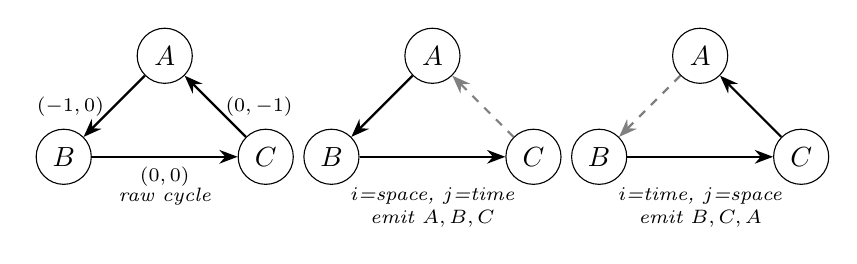
\begin{tikzpicture}[
    reg/.style={circle, draw, minimum size=7mm, inner sep=0pt},
    dep/.style={-{Stealth}, thick},
    stale/.style={-{Stealth}, thick, dashed, gray},
    node distance=11mm]
  % raw cycle
  \node[reg] (A1) {$A$};
  \node[reg] (B1) [below left=of A1] {$B$};
  \node[reg] (C1) [below right=of A1] {$C$};
  \draw[dep] (A1) -- node[left, font=\scriptsize] {$(-1,0)$} (B1);
  \draw[dep] (B1) -- node[below, font=\scriptsize] {$(0,0)$} (C1);
  \draw[dep] (C1) -- node[right, font=\scriptsize] {$(0,-1)$} (A1);
  \node[below=12mm of A1, font=\scriptsize\itshape] {raw cycle};

  % i=space, j=time
  \begin{scope}[xshift=34mm]
  \node[reg] (A2) {$A$};
  \node[reg] (B2) [below left=of A2] {$B$};
  \node[reg] (C2) [below right=of A2] {$C$};
  \draw[dep]   (A2) -- (B2);
  \draw[dep]   (B2) -- (C2);
  \draw[stale] (C2) -- (A2);
  \node[below=12mm of A2, font=\scriptsize\itshape, align=center]
    {$i$=space, $j$=time\\ emit $A,B,C$};
  \end{scope}

  % i=time, j=space
  \begin{scope}[xshift=68mm]
  \node[reg] (A3) {$A$};
  \node[reg] (B3) [below left=of A3] {$B$};
  \node[reg] (C3) [below right=of A3] {$C$};
  \draw[stale] (A3) -- (B3);
  \draw[dep]   (B3) -- (C3);
  \draw[dep]   (C3) -- (A3);
  \node[below=12mm of A3, font=\scriptsize\itshape, align=center]
    {$i$=time, $j$=space\\ emit $B,C,A$};
  \end{scope}
\end{tikzpicture}
\end{minipage}\hfill
\begin{minipage}[c]{0.36\textwidth}
\centering
\small
\begin{minipage}[t]{0.48\linewidth}
\centering
\textbf{$i$=space, $j$=time}
\begin{flushleft}\ttfamily\footnotesize
copy\ \ C $\to$ A\textsubscript{in}\\
A = F(A\textsubscript{in})\\
recv\ \ B\textsubscript{in} $\leftarrow$ A@$(i{-}1)$\\
B = G(B\textsubscript{in})\\
C = H(B)\\
send\ \ A $\to$ $(i{+}1)$
\end{flushleft}
\end{minipage}%
\hfill
\begin{minipage}[t]{0.48\linewidth}
\centering
\textbf{$i$=time, $j$=space}
\begin{flushleft}\ttfamily\footnotesize
copy\ \ A $\to$ B\textsubscript{in}\\
B = G(B\textsubscript{in})\\
C = H(B)\\
recv\ \ A\textsubscript{in} $\leftarrow$ C@$(j{-}1)$\\
A = F(A\textsubscript{in})\\
send\ \ C $\to$ $(j{+}1)$
\end{flushleft}
\end{minipage}
\end{minipage}
\caption{Left: the dependence graph of
Equations~\ref{eq:abc-a}--\ref{eq:abc-c} is a cycle (edges point from
producer to consumer and are labeled with their offsets). The space--time
mapping determines which edge is \emph{stale} (dashed): a purely temporal
offset refers to a value already resident from a previous timestep. Cutting
the stale edge leaves an acyclic graph. The topological order determines emitted statement order. Right: the ordering of statements changes under the two mappings. }
%The statement order flipsfrom $A,B,C$ to $B,C,A$; the stale dependence lowers to a register copy while the live cross-processor dependence lowers to a receive; and the tensor placed on the wire changes from $A$ to $C$. Under the $i$=time mapping, emitting $A$ first would overwrite the previous step's value of $A$ before $B$ reads it.}
\label{fig:dep-cycle}
\label{fig:emitted-ir}
\end{figure*}


\subsection{The shape of generated code}

The generated program is the same on every processor: a single loop over the
temporal dimension, whose body is a sequence of guarded statements. Each guard
is an \texttt{if} over the processor's spatial coordinates and the current
value of the temporal loop variable. The guards come from two sources: the
case structure implied by gimbal-locking (a statement written on a boundary
face such as $(i,i,k)$ only applies where $i=j$), and constraints the user
supplies directly (such as $i > j > k$). They are necessary because both the
temporal loop and the spatial processor grid range over the entire
iteration space: every processor reaches every timestep, but only some
$(\text{processor},\, \text{time})$ points lie inside a given statement's
region. The guard determines whether the current processor and timestep belong to the statement's guarded region.

Within one iteration of the temporal loop, each tensor of the recurrence
system owns one guarded block. A block contains everything that produces that
tensor's value for the current timestep: a receive if the value arrives from a
neighboring processor, a register read if it is already resident from a prior
timestep, and the kernel call that computes it. Sends are placed at the end of
the loop body, after all values for the step have been produced. The compiler must therefore determine an emission order for these blocks that respects their data dependencies.

\subsection{Breaking cyclic recurrence dependencies}
\label{sec:live-stale}


The order matters, and it cannot be read off the source program order, because the
dependence graph may be cyclic. Consider the following three-tensor system, which we use as a
running example (Figure~\ref{fig:dep-cycle}):
%
\begin{align}
  (i,j)_{A} &= F\big((i,\,j{-}1)_{C}\big) \label{eq:abc-a}\\
  (i,j)_{B} &= G\big((i{-}1,\,j)_{A}\big) \label{eq:abc-b}\\
  (i,j)_{C} &= H\big((i,\,j)_{B}\big)     \label{eq:abc-c}
\end{align}
%
$B$ depends on $A$, $C$ on $B$, and $A$ on $C$: a cycle
$A \to B \to C \to A$. $G$, $H$, and $F$ are functions. Taken at face value, the cyclic dependencies admit no valid emission order for the current timestep; an arbitrary order can produce incorrect code.

The cycle is broken by a space--time mapping. Once one dimension is declared
temporal, any dependence whose offset lies purely along the temporal
dimension refers to a value from a previous timestep. That value
already exists,  computed in an earlier iteration of the temporal loop
and is sitting in a register. It does not need to be produced during the
current step, so it imposes no ordering constraint on the current step's
code. We call such dependence edges \emph{stale}, and we remove them from the
ordering graph. The read itself is not removed; it is lowered to a
register read. Remaining edges, whose values are  produced during the current step,
are \emph{live}. Deleting stale edges leaves an acyclic graph. A
topological sort of the live edges yields a valid emission order.

In the example, map $i$ to space and $j$ to time. The dependence
$(i,j)_A \leftarrow (i,\,j{-}1)_{C}$ has offset $(0,-1)$: purely temporal, thus 
stale; the last step's $C$ is already in a register. The dependence
$(i,j)_{B} \leftarrow (i{-}1,\,j)_{A}$ has offset $(-1,0)$ and is purely spatial. It is hence live and this step's $A$, arriving from the neighboring processor. $(i,j)_C \leftarrow (i,j)_{B}$ has no offset and is live under any
mapping. Cutting the stale edge leaves the chain $A \to B \to C$, and the
emitted order is $A,\,B,\,C$.


The flipped mapping, with $i$ to time and $j$ to space, results in a different emitted order. Every offset keeps its
spelling but changes its meaning. The dependence $(i,j)_A \leftarrow (i,\,j{-}1)_{C}$  is now
\emph{spatial}, and the dependence  $(i,j)_B \leftarrow (i{-}1,\,j)_{A}$ is now \emph{temporal} and the source of the cut. %$C$ thus comes from a neighboring processor, so the edge$C \to A$ becomes live. The dependence on $(i{-}1,\,j)_{A}$ is now \emph{temporal}, not spatial as before. The last step's $A$ is already resident, so the edge $A \to B$ becomes stale. The cut thus moves to the other side of the cycle, 
The surviving chain is $B \to C \to A$, different than the original A,B,C order.

This reordering is necessary for correctness, not a stylistic choice. Suppose
we kept the source order $A,\,B,\,C$ under the flipped mapping. $B$'s
dependence on $(i{-}1,\,j)_{A}$ is stale: it must read the value of register
$A$ left over from the previous timestep. But the block for $A$ has
already run and overwritten that register with the current step's
value. $B$ silently consumes a value one timestep too new, resulting in incorrect output. The stale value must be read \emph{before} the operation that clobbers its register is emitted.

The topological sort in lines 3-11 of Algorithm~\ref{fig:algo} guarantees this. With $i$ mapped in time,  the stale edge $A \to B$ is deleted, its consumer $B$ loses its only incoming edge and
becomes a leaf of the ordering graph, so it is emitted
first, before the block that overwrites $A$. This is not a coincidence of
the example. The stale edge closes the cycle, so the surviving live edges
form a path from the stale edge's consumer ($B$) back around to its producer
($A$); any topological order of that path places the consumer before the
producer. In other words, sorting on live edges alone also enforces the
read-before-clobber constraint of the stale edge, for free.

The same structure appears at full scale in Cholesky. In this case the cycle
is $L_s \to L_c \to L_{gl} \to L_{gu} \to L_s$. The cut again changes with
the space--time mapping. The resulting topological orders correspond to the different compute orders required by the loop variants in Figure~\ref{tab:cholesky_variants}. %where the imperfectly nested variants require different relative orderings of the underlying compute statements (\textsc{potrf}, \textsc{trsm}, \textsc{syrk}, and \textsc{gemm}). 
The topological algorithm produces those orderings directly. Fixed traversals of the
source program (depth-first from any starting tensor) cannot produce correct orders for all mappings, because it must cut the cycle, and the correct cut is determined by the space--time mapping, not program order.

%The live/stale classification followed by a topological sort is the traversal that cuts in the right place by construction.

\subsection{Emitting Communication}
\label{sec:emitting-comm}


Once blocks are  lowered, cross-processor dependences are emitted as  receives. If $i$ is spatial, $(i,j)_X\leftarrow(i-1,j)_X$ means processor $i$ receives $X$ from processor $i-1$. The user does not write the corresponding send; the compiler inverts the relation and inserts a send from processor $i-1$ to $i$.
%Instead, the compiler inverts the receive relation and inserts the matching send into the source processor’s program. From the sender's point of view, processor $i$ sends $X$ to processor $i+1$, matching the receive. 


\begin{table*}[t]
\centering
\caption{Send synthesis in \textsc{DeducePushes}. Each receive
(\emph{dst}\,$\leftarrow$\,\emph{src}) is classified by its coordinate
and matched with a send.} %Same-base offset receives carry a window $\mathit{lo}\le i<\mathit{hi}$; comparing window length to the read \emph{stride} separates a \emph{relay} ($\mathit{hi}{-}\mathit{lo}>\text{stride}$) from a \emph{scatter} ($\mathit{hi}{-}\mathit{lo}\le\text{stride}$). Anchored and broadcast receives need no relay test, as they have pinned sources.}
\label{tab:send-taxonomy}
\small
\renewcommand{\arraystretch}{1.35}
\begin{tabular}{@{}lllll@{}}
\toprule
\textbf{Pattern} & \textbf{Receive \& window (dst\,$\leftarrow$\,src)} &
\textbf{Relay test} & \textbf{Originates at} &
\textbf{Send \& guard (src\,$\rightarrow$\,dst)} \\
\midrule
Temporal carry & $(i,j)\leftarrow(i,j{-}1)$ & --- & --- (register persists) & --- none; value stays resident \\
Systolic relay & $(i,j)\leftarrow(i{-}1,j),\ \ \mathit{lo}\le i<\mathit{hi}$ & $\mathit{hi}{-}\mathit{lo}>\text{stride}$ & receiver (each PE forwards) & $(i,j)\rightarrow(i{+}1,j),\ \ \mathit{lo}\le i{+}1<\mathit{hi}$ \\
Scatter (non-relay) & $(i,j)\leftarrow(i{-}\text{stride},j),\ \ \mathit{lo}\le i<\mathit{hi}$ & $\mathit{hi}{-}\mathit{lo}\le\text{stride}$ & each holder, one stride up & $(i,j)\rightarrow(i{+}\text{stride},j),\ \ \mathit{lo}\le i{+}\text{stride}<\mathit{hi}$ \\
Anchored       & $(j{+}1,j)\leftarrow(j,j)$ & --- & source PE & $(j,j)\rightarrow(j{+}1,j)$ \\
Broadcast      & $(i,j,k)\leftarrow(i,k,k)$ & --- & source PE (fan-out) & $(i,k,k)\rightarrow(i,j,k)\ \ \forall j$ \\
\bottomrule
\end{tabular}
\end{table*}


Table ~\ref{tab:send-taxonomy} shows how sends are synthesized, depending on the dependence.
Temporal dependencies require no send because the value remains locally resident.  Anchored receives such as $(j+1,j)_X \leftarrow (j,j)_X$ name the destination directly in terms of the source coordinate, so the source emits a send to $j+1$. Broadcasts such as $(i,j)_X \leftarrow (j,j)_X$  map many receivers $i$ to the same source $j$, so source $j$ emits sends to each receiver. Same-base offset receives like $(i,j)\leftarrow (i-1,j)$ require one additional test to check if receivers also forward the value (producing a systolic relay), or only receive.  

Consider a receive $(i,j)_X\leftarrow(i-stride,j)_X$  defined over the window $low \leq i < hi$. If $stride< hi-low$, then some receivers read from another point within the window, meaning some receivers also forward the value. If $stride \geq hi-low$, every sender remains outside the window, so receivers do not forward; this produces a scatter. Cyclotron uses scatters to construct recursive-doubling tree broadcast. 

The user never writes sends or send-side constraints. Cyclotron simply copies the receiver's if guards onto the synthesized send, ensuring the sender fires only when its destination is a receiver. Duplicate sends are suppressed when multiple rules would serve the same destination.

%a receive window lo≤i<hilo \textbackslash{}le i < hi with source i−stridei-\textbackslash{}textit\{stride\}, if stride<hi−lo\textbackslash{}textit\{stride\} < hi-lo, some receivers read from another point inside the window and therefore forward values onward; this is a relay. If stride≥hi−lo\textbackslash{}textit\{stride\} \textbackslash{}ge hi-lo, every source lies outside the receive window, so no receiver forwards a value; this is a scatter. Cyclotron uses scatters to construct recursive-doubling tree broadcasts. The compiler recovers those sends by classifying each receive's coordinate spelling (Table~\ref{tab:send-taxonomy}). Given a receive $(\textit{dst}\leftarrow\textit{src})$, when a slot on the source is spelled with a different base variable or a constant index---$(i,j,k)_{X}\leftarrow(i,k,k)_{X}$ or $(i,j,k)_{X}\leftarrow(i,0,k)_{X}$---the source is named absolutely, and the receive is a broadcast. The right-hand side is a lower-dimensional iteration space than the left-hand side, so the source is broadcast over the extra destination dimension. When the destination itself is spelled from the source's variable---$(j{+}1,j)_{X}\leftarrow(j,j)_{X}$---the hop is \emph{anchored}: the receiver sits a fixed distance from the source, and the send is emitted at the source, not forwarded by the receiver.

%A systolic relay and a scatter share the same syntax: both read a value a fixed stride away, $(i,j)\leftarrow(i{-}\text{stride},\,j)$ (Table~\ref{tab:send-taxonomy}). What separates them is whether anyone $\mathit{lo}\le i<\mathit{hi}$ where the user defined the receive. That window is a band of receivers along $i$; $\mathit{lo}$ and $\mathit{hi}$ are typically written in terms of $j$ (the source panel), as in $j\le i<j{+}\text{stride}$. If the stride is shorter than the window, some receivers sit far enough in that their source $i{-}\text{stride}$ is still inside the window. Those past nodes are themselves receivers, so they also send---they relay. Receivers at the front of the window, where $i{-}\text{stride}<\mathit{lo}$, still get the value rom outside; that first send is not a relay. If the stride is at least the window length, then $i{-}\text{stride}<\mathit{lo}$ for every receiver: nobody in the window reads from anybody else in the window. Every send comes from outside. That is a scatter: one-way, not a relay. Scatters are used to implement recursive-doubling tree broadcasts.

%The user never writes a send. The only guards in the program sit on the receive. The compiler copies that window onto the deduced send, shifted by the hop, so a send fires only when its destination is a receiver---the send-side inequalities in Table~\ref{tab:send-taxonomy}. A send whose destination falls outside the window is not emitted. When two patterns would serve the same receiver---an anchored hop composed with a relay, for example---the compiler also suppresses the extra send, so exactly one sender fires.

\subsection{Minimizing communication}
\label{sec:block-cyclic}

%Triangular iteration spaces such as Cholesky's are inherently load-imbalanced under a one-tile-per-processor mapping. The standard remedy is a 2D block-cyclic decomposition, which assigns the tiled iteration space to a smaller physical grid in round-robin fashion, so each physical processor hosts several \emph{virtual} processors and thus several blocks of work. This has two benefits. It smooths the triangular imbalance, and it deduplicates communication: when the physical grid is smaller than the virtual grid, a tile broadcast along a row need not be received once per virtual processor. Once a resident virtual processor has the tile, the others on the same physical processor reuse it rather than require it's own separate message. Cyclotron applies the decomposition as a simple post-processing pass over the generated code: it wraps each processor's program in two additional loops ranging over its resident virtual processors, and injects the guard and modulo-index logic that routes work to the right virtual processor. 

Triangular iteration spaces like Cholesky’s are load imbalanced under a one-tile-per-processor mapping. Cyclotron therefore supports a 2D block-cyclic decomposition, which maps the virtual processor grid onto a smaller physical grid in round-robin fashion. This both balances work and exposes redundant communication. If several virtual processors on the same physical processor require the same tile from another processor, only one network receive is necessary and the remaining consumers/virtual processors  can reuse the same local copy. Cyclotron applies this decomposition in two phases. The first is a post-processing pass that wraps each processor program with loops over its resident virtual processors and inserts the required modulo and guard logic. Afterwards, the generated code is specialized to each physical processor; control flow is removed, as well as redundant sends, receives, and guards. The resulting per-processor programs remain small because each generated operation corresponds to a coarse-grained tiled computation. An alternative is to eliminate redundant communication with a runtime cache, but this introduces additional runtime overhead.


%Cyclotron removes redundant transfers using either a runtime cache or compile-time partial evaluation. The runtime cache converts duplicate receives into local reads, while partial evaluation specializes each physical processor's program by unrolling loops and statically removing redundant sends, receives, and guards. The latter reduces runtime control-flow overhead at the cost of larger generated programs. Partial evaluation is most useful for smaller tiles, where control-flow overhead is non-negligible. The resulting code size depends on the number of generated loop iterations rather than the tile dimension itself, and remains manageable because each unrolled iteration still corresponds to a coarse-grained tiled operation rather than scalar computation. In our evaluated configurations, the specialized per-processor programs remain only on the order of kilobytes.




%The redundant transfers are de-duplicated by one of two general mechanisms, which the user selects and which trade off against tile size. A \emph{runtime cache} logs, during execution, which tiles a physical processor has already received, turning duplicate receives into local reads; it leaves the single shared, guarded program intact. An alternative \emph{partial-evaluation} compiler pass instead specializes that program into a distinct program per physical processor at compile time: it evaluates the loops and the rank- and timestep-comparison guards, removing control flow, and then statically elides the redundant sends and receives. Removing the guards pays off when tiles are small, where the per-tile control-flow overhead is a tangible fraction of the modest compute each tile carries; it is negligible when tiles are large, and there the runtime cache is preferable. The cost of the static pass is a larger compiled program: partial evaluation unrolls each processor's loops over its resident blocks into straight-line code, so the program grows with the block-cyclic factor---the number of blocks per processor---and is independent of the tile dimension. We note that the loops unrolled are over large blocked operations, keeping the size of unrolled code manageable (kilobytes). This pass has the secondary benefit of eliminating the need to evaluate control flow, which can become tangible if tile sizes become extremely small. By default, we always use partial evaluation. Without such abstractions, writers of MPI code must reason about de-duplication manually. 

\section{System and Implementation}

The Cyclotron front-end language and compiler are implemented in Python, while the runtimes that execute generated programs are native C++ and Rust. Cyclotron has three backends: a C++ backend for CPU clusters, a C++ backend for GPU clusters, and a Rust backend built with DAM \citep{zhang2024dataflow}, a framework for modeling dataflow architectures in which PEs communicate over channels. Each backend interprets the same portable Protobuf program, allowing a generated executable to run unchanged across backends. The Rust backend is used primarily for simulation. It reproduces the communication behavior of the cluster backends, including simulated MPI protocol behavior, without requiring payloads. This allows Cyclotron to detect indefinite hangs and model communication and kernel latencies without executing on a cluster. The simulator can also execute with real payloads and produce correct results, although this mode is disabled by default because it runs on a single processor. The Rust backend can be used to simulate spatial-processors composed of interlinked PEs; this exploration is future work.
%The Cyclotron front-end language and compiler is embedded in Python, but the underlying runtimes that execute the programs are native (C++ and Rust). Cyclotron itself has three backends; a C++ backend for CPU clusters, a C++ backend for GPU clusters, and a Rust backend that simulates distributed execution of processing elements. Each backend is an interpreter that executes every instruction of the program. These generated programs themselves are portable Protobuf files, allowing the same generated program to run unchanged across backends. Input data can either be baked into the program, or created by the runtime during execution. The Rust backend is used for solely simulation purposes; it sends the same messages as a cluster would, but is intended to run without payloads, simply to model the communication with simulated MPI protocols. It can be used to identify MPI deadlocks without having to run the program on an MPI cluster. Communication latencies and kernel cycles can run with simulated latencies. The Rust backend can still compute valid results with actual message payloads, but this is turned off by default as it runs on a single processor.

%Static compiler-generated schedules are competitive with, and at small per-rank tile counts beat, a mature task-based runtime (DPLASMA/PaRSEC); the residual gap at high tile-counts is attributable to runtime overlap mechanisms (multi-stream, dedicated progress thread) that are orthogonal to schedule generation."

\section{Evaluation}
\label{sec:eval}
We evaluate performance on CPU and GPU clusters. Both are hosted on Perlmutter, a supercomputer at Lawrence Berkeley National Laboratory. GPU experiments use 16 A100 GPUs, four per node, connected by NVLink within a node and HPE Slingshot 11 across nodes. CPU experiments use 16 Perlmutter nodes connected by Slingshot. 
%We compare Cyclotron against Cray ScaLAPACK on CPUs and SLATE and cuSolverMp on GPUs. Cyclotron and the corresponding baseline use the same input sizes, floating-point precision (FP32), tile sizes, BLAS/LAPACK implementations, and CPU OpenMP thread counts. GPU kernels use cuBLAS/cuSOLVERDn, CPU kernels use Cray LibSci, and communication uses MPI. This controls for kernel performance so that measured differences primarily reflect communication scheduling and orchestration. 
We compare against Cray ScaLAPACK, SLATE, and cuSolverMp using matched precision, tile sizes, BLAS/LAPACK kernels, thread counts, and MPI communication. Each configuration uses two warmups and four measured trials; we report the best runtime.
%We evaluate Cyclotron programs on three back-ends: CPU-based clusters, GPU-based clusters, and the Rust simulator built with DAM \citep{zhang2024dataflow}, a framework for modeling dataflow architectures in which PEs communicate over channels. Our GPU cluster is composed of 16 Nvidia A100 GPUS, 4 per node, with GPUs communicating over NVLINK within nodes and over HPE Slingshot 11 between nodes. Unless noted, the CPU cluster is 16 nodes, all communicating over Slingshot. We compare performance against Cray ScaLAPACK, the standard distribution for performing high performance linear algebra on CPUs, as well as its GPU successor, SLATE. Underlying BLAS/LAPACK kernel calls go through CUBLAS/CuSolverDn on GPUs and MKL on CPUs, and all communication over MPI. Within each experiment, we ensure that all Cyclotron comparisons against SLATE and ScaLAPACK link against the same version of the  MKL and CUBLAS/CuSolverDn libraries (with thread counts set equivalently) to ensure that speedups arise from differences in communication scheduling, not the speed of the kernels. Comparisons of Cyclotron vs SLATE and Cyclotron vs ScaLAPACK use the same input sizes, floating point precision (fp32), tile sizes, and CPU OpenMP thread counts to ensure fair comparisons. Each experiment runs long; for each speedup number for each tested framework, we do 2-warm up iterations, and then take the best of 4 trials.

%Both block-cyclic and non-block-cyclic decompositions are valid targets. When input data is already sharded non-cyclically, a non-block-cyclic run avoids a reshard; when it is sharded block-cyclically, the block-cyclic path matches it directly. For every comparison against a library we hold the block-cyclic factor---the number of blocks per physical processor---identical on both sides, an apples-to-apples comparison; and where the comparison is itself about block-cyclic performance, we additionally sweep ScaLAPACK's own block-cyclic factor so the baseline is reported at its best. Because small tiles perform best for both Cyclotron and ScaLAPACK, our evaluation uses small tiles throughout and therefore the partial-evaluation pass; the compiled kernel is reusable across runs and inputs. That pass's code-size cost is negligible next to the data. Weak-scaled at block-cyclic factor $c = 16$ with a $256$ tile, the serialized per-process program (excluding the baked matrix tiles) averages $169$~KiB across our eleven Cholesky topologies on a $4{\times}4$ physical grid and $341$~KiB on an $8{\times}8$ grid, against a $64$~MiB matrix slice per process---a $190$--$390\times$ gap, and $110\times$ even for the largest program (the broadcast topology). Because the program is byte-identical across tile sizes while the matrix slice grows with the square of the tile, the gap widens past $10^{4}\times$ at the $2048$ tiles of our GPU runs.
% Caveats if challenged: static-dedup programs at c=16; 64 MiB is the dense
% N^2/P share (owned lower triangle ~32 MiB, still ~100-190x); program bytes
% are protobuf op records, a proxy for instruction footprint, not machine code.

\subsection{Comparing Communication Strategies}
\label{sec:eval-comm}



\begin{figure*}[t]
\centering
\begin{subfigure}{0.49\textwidth}
\centering
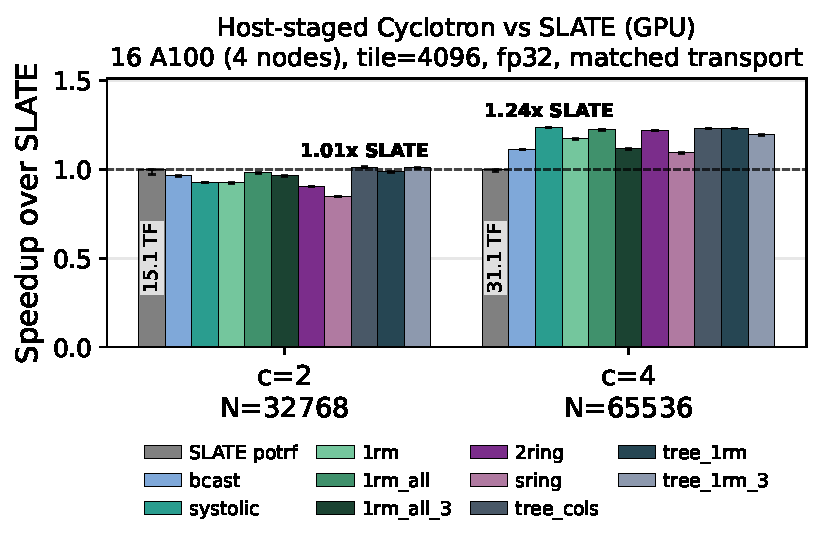
\includegraphics[width=\linewidth]{fig_gpu_vs_slate_bounce_t4096.pdf}
%\caption{Tile $2048$.}
\label{fig:gpubc-slate-t2048}
\end{subfigure}
\hfill
\begin{subfigure}{0.49\textwidth}
\centering
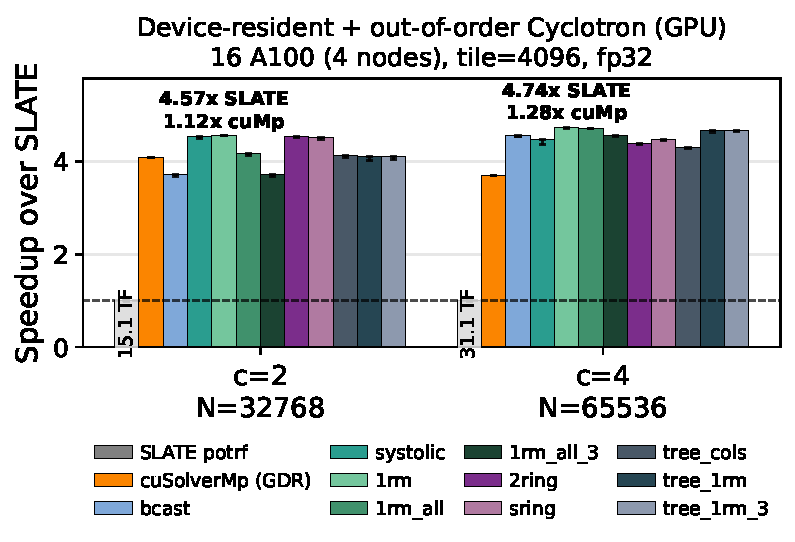
\includegraphics[width=\linewidth]{fig_gpu_vs_cusolvermp_portd_t4096.pdf}
%\caption{Tile $4096$.}
\label{fig:gpubc-slate-t4096}
\end{subfigure}
%\caption{Block-cyclic Cholesky on four GPU nodes ($16$ A100s, one rank per GPU, so a fixed $P{\times}P$ process grid with $P{=}4$): speedup over SLATE with block-cyclic factor $c\in\{2,4\}$, at tile size $2048$ (left) and $4096$ (right). Each process owns $c{\times}c$ tiles, so the global dimension is $N=P\,c\cdot\text{tile}$; SLATE uses the same tile as its block size.  Whiskers denote median time.}
\caption{Block-cyclic Cholesky on four GPU nodes ($16$ A100s, 1 rank/GPU,
so $P{=}4$): 
Left: speedup over SLATE, with host-staged communication.  Right: speedup over Nvidia cuSolverMp and SLATE, with device-device direct communication.
tilesize=$4096$, with block-cyclic factor $c{=}2$ and $c{=}4$ (right). Each
process owns $c{\times}c$ tiles, so $N=P\,c\cdot\text{tile}$; SLATE and
cuSolverMp use the same block size ($=$tile) and the same $c$. Bars are the
fastest steady cycle; whiskers reach  slowest.}
\label{fig:gpubc-slate}
\end{figure*}

\begin{figure}[t]
\centering
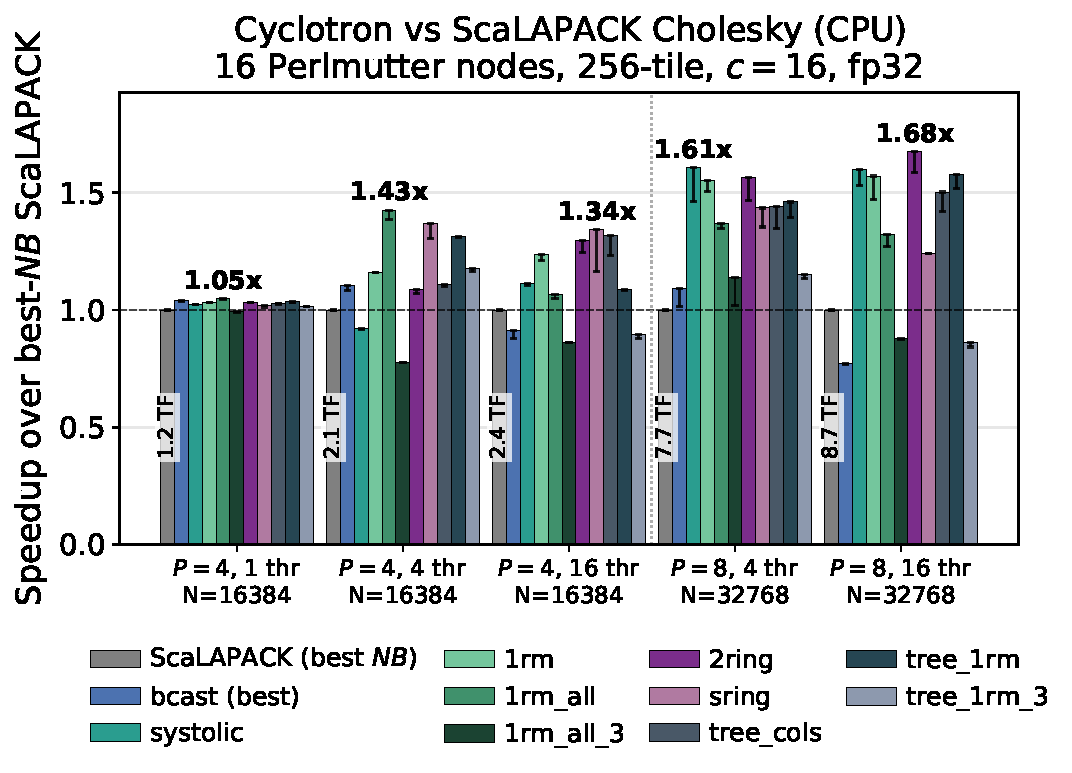
\includegraphics[width=\columnwidth]{bc16av_speedup2.pdf}
\caption{Cyclotron Cholesky speedup over ScaLAPACK on 16 CPU nodes. \(P\times P\) ranks, tilesize=256, 16 tiles/rank; “thr” denotes threads/rank. Whiskers show run-time variation}
%\caption{Speedup over ScaLAPACK on 16 CPU nodes, using $P{\times}P$ ranks, ``thr''=threads/rank. ScaLAPACK's block size $NB$ was swept; the best (256 in all cases) is the baseline, resulting in c=16. We also set Cyclotron $NB{=}256$. The best communication pattern varies with the rank count, threads/rank, and problem size. Whiskers denote the slowest and fastest runs.}
\label{fig:bc16av}
\end{figure}

\begin{figure}[t]
\centering
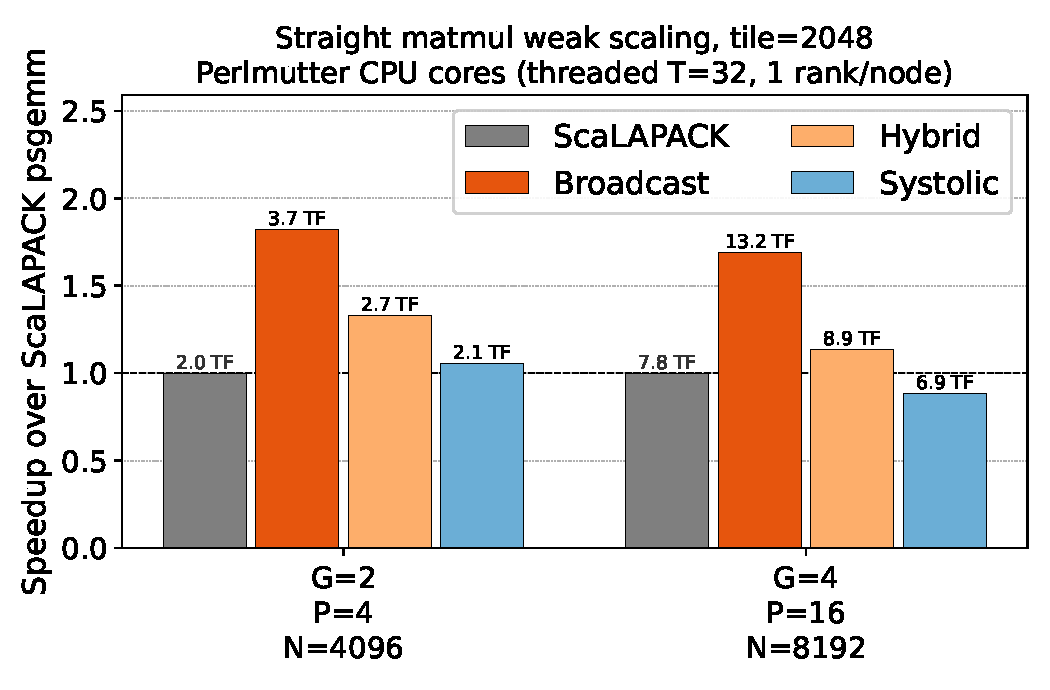
\includegraphics[width=\columnwidth]{matmul_perlmutter_straight.pdf}
\caption{Cyclotron GEMM vs. ScaLAPACK on 4 and 16 CPU nodes, with systolic, broadcast, and hybrid schedules}
\label{fig:matmulRes}
\end{figure}

For a specific program, the best communication schedule is rarely fixed; the fastest one will depend on factors including the network topology and processor architecture (CPUs vs GPUs), in addition to tile size, tiles per rank, and input size. The relative performance of schedules also changes; we observed a single schedule can perform over twice as fast as an alternative on CPUs, while the alternative often performs faster than the other on GPUs.

We compare a sample set of eleven Cyclotron Cholesky variants that differ only in communication strategy, including broadcasts, systolic relays, 2-rings, bidirectional split-rings (sring), modified rings (1rm), and trees, against ScaLAPACK and SLATE. We use an $ij$ spatial mapping here because it enables communication deduplication, which is fundamentally not possible in other Cholesky spatial mappings.

%We therefore compare a sample set of eleven different Cycltron Cholesky programs, varying only in terms of their communication strategy, to both each other and to the hand-optimized Cholesky kernel in Scalapack and SLATE. Our 11 Cyclotron programs include permutations of broadcasts, systolic, modified rings, srings, 2rings, and tree broadcasts.  

\paragraph{CPU Results} Figure~\ref{fig:bc16av} compares 11 Cyclotron Cholesky communication schedules against ScaLAPACK on 16 CPU nodes using \(P\times P\) grids, \(P\in\{4,8\}\), with 4 or 16 threads/rank. We also include an effectively serial control (\(P=4\), 1 thread/rank), where communication choice has little effect and all Cyclotron schedules perform similarly to ScaLAPACK.

ScaLAPACK's block size \(NB\) was swept; the best was \(256\) in all cases, which we use as the baseline. Cyclotron also uses \(NB=256\), giving \(c=16\). As per-rank computation becomes more parallel, communication becomes increasingly important: some schedules perform worse than ScaLAPACK, while the best Cyclotron schedule achieves \(1.34\)--\(1.68\times\) speedup across the remaining configurations. The winning communication strategy also changes with the configuration, and schedules that perform well in one regime can perform poorly in another. This demonstrates that communication policy becomes a first-order performance choice once computation is sufficiently optimized.
The choice of communication policy is also heavily machine dependent. On Perlmutter's 16 nodes, the broadcast policy performed poorly. However, on a separate 4-node  machine (with nodes connected via InfiniBand), the broadcast schedule was universally best. We postulate this is due to the 4-nodes being densely connected, making 1 to all broadcasts practical. 

%\paragraph{CPU Setup:} Figure ~\ref{fig:bc16av} compares eleven different communication schedules on a 16 node CPU cluster, with three logical configurations of ranks and threads to show its affect on the best schedule; 1 rank/processor with 4 threads/rank, 4 ranks/processor with 8 threads/rank, and 4 ranks/processor with 16 threads/rank. For each configuration, we use an equivalent block cyclic decomposition and tile size for Cyclotron, to ensure runtime comparisons between ScaLAPACK and Cyclotron come from differences in the underlying communication policy and the runtime that issues communication and kernels. We further confirm that ScaLAPACK and Cyclotron call the use the version of MKL for the underlying math calls. 

%In each configuration, the best Cyclotron schedule substantially outperforms the hand-optimized ScaLAPACK, while a few (like the 1 to all broadcast) perform substantially worse. More importantly, in each configuration a different Cycltron schedule comes out on top. Using a depth-2 modified rink for each communication channel dominates at 1 rank per node. In the second configuration, the purely systolic variant wins. In the third, the 2ring wins, which is systolic in the vertical dimensions but uses a 2ring for the horizontal dimension. This 2-ring strategy in turn  performed very poorly in the first regime. Notably the 1-all broadcast behaves poorly here, even though on our GPU backend it performs exceptionally well. All speedup claims and per-point winners are preserved when using the median to determine speedup, except at $P{=}4$/16-thread where the top two topologies are within run-to-run variance. 

%It is extremely hard to explain why a particular certain schedule dominates in a certain regime, because it's dependent on so many factors. This shows the importance of trying different communication policies, which amount to single line changes in Cyclotron user programs. ScaLAPACK's communication, on the other hand is fixed; a broadcast tree for vertical communication and an sring for horizontal communication. 

%\paragraph{GPU Setup:} Figure ~\ref{fig:gpubc-slate} shows the same 11 communication schedules but for 6 different configurations on a 16 GPU system. In this experiment, we keep tile sizes large (2048 and 4096) to keep the GPUs busy. The baseline aggregate teraflops is labeled; for our largest problem size, we observe SLATE achieves 31.1 teraflops of fp32, about 10\% of the aggregate peak compute bandwidth of 16 A100s. This makes sense; a Cholesky on a single GPU (without any load imbalance or communication) will not achieve even half an A100's peak performance. We do not vary the number of ranks per node or OpenMP threads/rank (as we do in the CPU experiment), because it is typical to assign 1 rank and thread per GPU; all computations run on the GPUs. We instead vary the block-cyclic factor c, such that each GPU handles $c \times c$ blocks of work, which are assigned to the GPUs round-robin. 

%\paragraph{GPU Results.} Figure~\ref{fig:gpubc-slate} evaluates the same eleven communication schedules across six configurations on 16 GPUs. We use large matrix tiles (2048 and 4096) to keep the GPUs well utilized. The baseline aggregate throughput is labeled; at the largest problem size, the SLATE baseline achieves 10\% of the aggregate peak throughput of 16 A100s. Unlike the CPU experiments, we fix one MPI rank and one host thread per GPU, since all computation executes on the GPUs. We instead vary the block-cyclic factor \(c\), so that each GPU hosts \(c\times c\) virtual processors assigned round-robin.

\paragraph{GPU Results.}
Figure~\ref{fig:gpubc-slate} (left) compares Cyclotron against SLATE using host-staged communication on 16 A100 GPUs. We use tile size 4096 and evaluate block-cyclic factors \(c=2\) and \(c=4\). We use host staging here because SLATE (on Perlmutter) does not support GPU-direct communication, giving both systems the same communication path. Under this matched transport, Cyclotron is competitive with SLATE at \(c=2\) and reaches up to \(1.24\times\) SLATE at \(c=4\). The relatively smaller spread among Cyclotron's communication schedules contrasts with the CPU results; the importance of communication strategy is architecture dependent.

Figure~\ref{fig:gpubc-slate} (right) evaluates Cyclotron on 16 A100s with device-resident GPU-direct communication and out-of-order execution, and compares against Nvidia cuSolverMp, which likewise uses GPU-direct communication. Cyclotron reaches \(4.57\times\) and \(4.74\times\) SLATE, and \(1.12\times\) and \(1.28\times\) cuSolverMp. %for \(c=2\) and \(c=4\), respectively. 

The difference with cuSolverMp appears to come largely from execution scheduling. cuSolverMp is closed source, but profiling shows that its communication is performed using NCCL broadcast collectives, with communication and computation proceeding in bulk-synchronous stages. Cyclotron instead emits dependency-driven code that naturally overlaps communication and computation, and out-of-order execution further increases this overlap. %These results suggest that Cyclotron's advantage comes from exposing and exploiting a more flexible communication and execution schedule.

%Here, unlike in the CPU experiments, the 1-all communication strategy performs exceptionally well in each configuration. It is the fastest except for the largest problem size, where tree\_1rm wins, which uses a modified ring for the broadcast of $Lc$ and a depth-2 modified ring otherwise. We postulate this is due to the presence of a dense NVLINK topology connecting each locale of 4 GPUS; 1 to all broadcasts make more sense because within each locale, each GPU is connected to each GPU as a peer. In the CPU cluster, data between the 16 nodes must always cross a node boundary. 

\paragraph{CPU Matrix Multiply.} We also evaluate three different matrix multiply schedules against ScaLAPACK on our 16-node CPU backend. We compare systolic, broadcast, and hybrid schedules (broadcast in 1 dimension, systolic in the other). Figure ~\ref{fig:matmulRes} shows the broadcast variant working best.


%There is one configuration in which SLATE outperforms Cyclotron, a non-block cyclic program (c=1, N-16284, tile-size=4096), where we achieve .93x the performance of SLATE. We also note that speedups over SLATE (1.04x-1.35x) are smaller than our speedups over ScaLAPACK (1.43x-1.68x). We postulate this is due to a large swatch of modern SLATE features not implemented in Cyclotron, particularly a dynamic DAG scheduler, as well as lookahead (a common optimization for solvers), which both help alleviate load balance. These optimization kick in here because c=1 is inherently load-imbalanced; c=1 means there is no block-cyclic decomposition. We note that while most modern workloads choose a block-cyclic decomposition (c>1) when possible, c=1 is still a viable workload, especially if input data was not pre-sharded over processors in a block-cyclic way. Nevertheless, the speedup over SLATE likely comes from the same mechanism as that over ScaLAPACK; SLATE hardcodes it communication schedule (a tree broadcast), whereas we can explore the space. We leave dynamic DAG scheduling and lookahead as future work. 

%From inspection of ScaLAPACK source, we postulate the differences between ScaLAPACK and Cyclotron are explainable by the difference in order of operations and communication strategy chosen.   The block cyclic decomposition assigns 16*16 blocks of work per rank. It continues by batching together the execution of the same operation from each block, before moving to the next operation. This means if each block starts with a send, then it issues 16x16 sends at once. Cyclotron operates differently; it executes all operations from 1 block before moving to the next. This means send, compute, and receive operations get interleaved. 


%\paragraph{Setup.} We weak-scale a blocked Cholesky factorization: each processor owns one $2048 \times 2048$ tile, so $N = 2048\,G$ on a $G \times G$ grid ($P = G^2$, up to $64$ processes on four nodes, one single-threaded MKL rank per core). The baseline is ScaLAPACK's \texttt{pspotrf} with block size $NB = 2048$, matching our one-tile-per-process distribution. This $NB$ is larger than ScaLAPACK's customary $64$--$256$ and penalizes its unblocked panel factorization (\texttt{pspotf2}), but it holds the data distribution constant across all systems. The Netlib source shows that this distribution hardcodes several broadcast strategies---a systolic ring, a multi-ring, and a tree---yet the communication configuration is fixed for the user: \texttt{pspotrf} sets a split ring (\texttt{S-ring}) along process rows and the default 1-tree / \texttt{MPI\_Bcast} down process columns, calls that sit inside the factorization and are not arguments the user can set. The Cyclotron variants all run the same compute kernels and the same schedule; they differ only in the communication recurrences given for the three inter-processor \emph{actions} of Figure~\ref{fig:tensor_constraints}---the \textsc{trsm} panel $L_{gl}$ along rows, and the transposed panel $L_{gu}$ and diagonal factor $L_c$ down columns. Those are three actions on two axes: $L_{gu}$ and $L_c$ share the column direction but need not share a topology. Each variant is a handful of lines in the notation of Section~\ref{sec:communication}: pure broadcasts, pure systolic relays (under both the $k$-temporal and $k$-spatial mappings), LINPACK's modified increasing ring and increasing-2-ring, and a depth-3 extension of the modified ring that sends directly to the first \emph{three} neighbors before relaying. No compiler, runtime, or kernel code changes between variants.

%\paragraph{No single strategy dominates.} Figure~\ref{fig:chol-comm} shows speedup over ScaLAPACK at each grid size. At small scale the broadcast wins decisively ($1.79\times$ at $P=4$, $1.37\times$ at $P=9$): fan-out is cheap when there are few consumers, and the panel arrives everywhere in one step. As $P$ grows, weak scaling shifts the bottleneck to the chain of dependent panel factorizations along the diagonal, and the piecewise rings take over: the modified ring applied to all three flows leads from $P=16$ onward, and deepening its direct-send prefix from two hops to three extends the lead ($1.15\times$ at $P=16$, $1.04\times$ at $P=64$). The crossover is the point: the best communication schedule is a function of scale, so a library that hardcodes one strategy necessarily leaves performance behind at some operating points.

%\paragraph{The wins come from the critical path.} The progression at $P=64$ isolates where the time goes. The plain systolic relay trail  ScaLAPACK by $14\%$; replacing the panel's row relay with the modified ring recovers to $-8\%$; applying the ring to the column flows as well reaches $-3\%$; and deepening the ring to three direct hops finishes $4\%$ \emph{ahead}. Each step is a DSL-only edit, and each works for the same reason: the direct hops deliver the panel to exactly the processors whose \textsc{trsm} and \textsc{potrf} work begins next, removing relay hops from the diagonal critical path. The two-ring, by contrast, is a wash at every scale---its direct hop lands at the \emph{midpoint} of the remaining processors, which shortens time-to-last-receiver but not the diagonal chain, and the critical path here is the chain. Which pattern helps is thus a property of the algorithm's dependence structure, not of the pattern---a second reason the choice belongs in the program text rather than in the library.

%\paragraph{Expressivity is the enabler.} ScaLAPACK and HPL pick a topology per \emph{dimension of the process grid}. Cyclotron picks one per \emph{communication action}---and a recurrence system has as \emph{many} actions as it has cross-processor reads, not as \emph{few} as the grid has axes. In Cholesky that is the difference between ``rowwise S-ring, columnwise tree'' and giving $L_c$, $L_{gu}$, and $L_{gl}$ three independent communication policies, two of which travel the same axis. The modified ring and the two-ring exist in HPL's menu, but only as the panel broadcast, not as a per-action choice; the depth-2 ring that deploys the strategy for all three communication actions (and outperforms Scalapack and our other variants in one experiment) is expressible in neither.  Here each of those is a simple modification of the communication recurrences (Section~\ref{sec:communication}), which is what makes searching the space practical.

\subsection{Generating Different Spatial Mappings}
\label{sec:eval-schedules}




\begin{figure}[t]
\centering
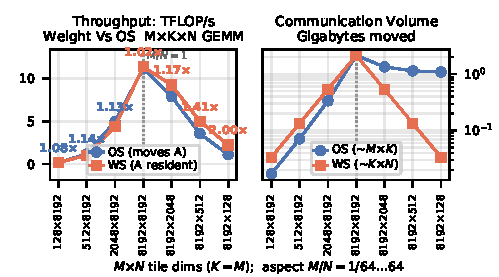
\includegraphics[width=\columnwidth]{ws_vs_os_asym_P4_16node_full.pdf}
\caption{Weight-stationary (\(ik\)-spatial) versus output-stationary (\(ij\)-spatial) GEMM on 16 CPU nodes. As \(N\) decreases relative to \(M=K\), weight-stationary increasingly wins by keeping the larger \(A\) tiles stationary.}
\label{fig:WSvsOS}
\end{figure}

The space--time annotation of Section~\ref{sec:notation} is a retag, not a
rewrite. The same blocked triangular-solve recurrences produce two complementary
wavefronts depending on which index is spatial: an $i$-spatial  pipelines the solution $X$, while a $k$-spatial pipelines the right-hand side $B$. Each leaves a  region of processors idle while waiting for its wavefront, but these idle regions are complementary. One can therefore interleave the two mappings by changing only the space--time annotation between successive right-hand-side chunks.


%Each wavefront leaves a triangular idle region---processors wait for the front to arrive---and the two idle triangles are complementary. Interleaving the two schedules, which Cyclotron emits from the same kernel by flipping the annotation and remapping the spatial index between loops, fills one triangle with the other's work. 

%A single isolated wavefront occupies $2P-1$ steps of which only $P(P+1)/2$ are busy; the
%interleaved pair occupies $P+1$ busy steps per problem and so has analytic
%throughput bound $2P/(P+1)$ over back-to-back isolated runs ($1.60\times$ at
%$P=4$, $1.78\times$ at $P=8$, approaching $2\times$ as $P$ grows).

\begin{table}[t]
\centering
\caption{Blocked \textsc{trsm} throughput on four CPU nodes
(Perlmutter), tile $1024\times1024$, $1024$ right-hand sides).
Entries are GFLOPS/proc. Overlap is ping-pong time against the sum of the
two isolated systolic times. ScaLAPACK is \texttt{pstrsm} on the same
$P{\times}1$ grid and the same number of solves (20)}
\label{tab:trsm-pingpong}
\small
\begin{tabular}{@{}l r r@{}}
\toprule
 & $P=4$ (1/node) & $P=8$ (2/node) \\
\midrule
$i$-spatial systolic & 54.37 & 49.95 \\
$k$-spatial systolic & 54.54 & 50.36 \\
broadcast & 55.70 & 51.86 \\
modified ring (1rM) & 55.39 & 50.75 \\
increasing 2-ring & 55.92 & 49.89 \\
ping-pong systolic & \textbf{93.65} & \textbf{91.98} \\
ScaLAPACK \texttt{pstrsm} & 47.55 & 44.33 \\
\midrule
overlap speedup & $1.72\times$  & $1.83\times$ \\
vs.\ ScaLAPACK & $1.97\times$ & $2.07\times$ \\
\bottomrule
\end{tabular}
\end{table}


Table~\ref{tab:trsm-pingpong} evaluates this ``ping-pong'' schedule. Even-numbered chunks use one spatial mapping and odd-numbered chunks use the other, allowing work from one wavefront to fill much of the other's pipeline imbalance. In isolation, the Cyclotron variants perform similarly: changing the spatial dimension or replacing a systolic relay with a broadcast, modified ring, or 2-ring has little effect on the critical path of a single solve. Interleaving the two complementary systolic mappings, however, improves throughput by \(1.72\times\) at \(P=4\) and \(1.83\times\) at \(P=8\) relative to running them back-to-back, reaching \(1.97\times\) and \(2.07\times\) the throughput of ScaLAPACK. The ping-pong throughput remains similar across the two placements (93.65 vs.\ 91.98 GFLOPS/proc), indicating that the benefit does not arise merely from packing multiple ranks onto a node.

%\paragraph{Setup.} We execute a blocked \textsc{trsm} $LX = B$ on the same four-node InfiniBand cluster as Section~\ref{sec:eval-comm}: one $1024\times 1024$ $L$ tile and a $1024$-column right-hand side per processor., so $M = 1024\,P$.  Ranks are spread across nodes ($P=4$ is one rank per node; $P=8$ is two), every ring neighbor is an InfiniBand hop, and each rank is a single MKL thread.  Each isolated Cyclotron variant runs ten solves. Ping-pong interleaves ten of one mapping with ten of the other (twenty solves), and ScaLAPACK runs twenty \texttt{pstrsm} calls to match that pair. Overlap speedup is $(t_{i}+t_{k})/t_{\mathrm{pp}}$: the two isolated tens, run separately and added, are the back-to-back baseline for the twenty ping-ponged solves. The table reports GFLOPS/proc for Scalapack and four Cyclotron programs---$i$-spatial systolic, $k$-spatial systolic, an $i$-spatial broadcast of $X$, modified ring, a 2-ring, and the ping-pong interleaving of the two systolic programs. ScaLAPACK is \texttt{pstrsm} on a matching $P{\times}1$ process grid with block size $NB = 1024$. Every number is the best of five timed runs after one warmup.

%Table~\ref{tab:trsm-pingpong} shows the result of using both spatial systolic schedules in tandem. Our TRSM kernel processes a chunk of right hand-sides at a time so we execute a ping-pong strategy where even numbered chunks are processed with one spatial mapping and odd chunks sides with the other, causing the pipeline imbalances of each spatial kenrnel to perfectly balance each other out. The isolated Cyclotron variants sit together; flipping $i$ for $k$, or a systolic relay for a broadcast or modified of 2-ring does not change the critical path of a single solve, so none of them beats the others by much, and none of them beats ScaLAPACK by more than about $1.5\times$. Interleaving the two systolic Cyclotron programs (ping-pong) nearly doubles that throughput---$1.70\times$ at $P=4$ and $1.72\times$ at $P=8$ over running them back to back.
%---and lands at $97\%$ of the $P=8$ Against ScaLAPACK the same schedule is $2.47\times$--$2.55\times$ faster. The absolute ping-pong rate is stable across the two placements ($78$ vs.\ $73$~GFLOPS/proc), so the overlap  is not an artifact of packing ranks onto one node.


Figure~\ref{fig:WSvsOS} compares two spatial mappings of the same systolic matrix multiply and shows that the better mapping depends on tile shape. We compute $C=AB$ on a $4\times 4$ processor grid, where $A$ is $M\times K$, $B$ is $K\times N$, and $C$ is $M\times N$. We fix $M=K$ (square $A$ tiles) and sweep $N$. When $M=K=N$, both dataflows perform equivalently. As $N$ shrinks, $A$ becomes much larger than $B$ and $C$: the output-stationary mapping moves $A$ and $B$, whereas the weight-stationary mapping keeps the larger $A$ tiles fixed and moves only the smaller $B$ and $C$ tiles. Consequently, the weight-stationary mapping outperforms output-stationary as $N$ decreases.


%As $N$ shrinks, square tiles of $A$ become much larger than the tall, skinny tiles of $B$ and $C$. An output-stationary systolic $ij$ mapping moves tiles of $A$ and $B$ and keeps $C$ in place, whereas a weight-stationary systolic $ik$ mapping fixes the larger $A$ tiles and only moves the smaller $B$ and $C$ tiles. The figure shows that as $N$ shrinks, the weight-stationary variant dominates.

\subsection{Fusion}
\label{sec:eval-fusion}

%Another way to fuse kernels is explicitly, by writing both programs on the same iteration space. A typical use case for such fusion is a Cholesky decomposition followed by a triangular solve. A blocked Cholesky factorization produces each $L$ tile at a known panel iteration; a forward substitution $Ly = b$ consumes that tile the moment it exists. Writing he solve recurrences on that same panel---$y_j$ relayed down the factor column, the row partial summed east---pipelines the solve behind the factorization. ScaLAPACK cannot do this: \texttt{pspotrf} (Cholesky) and \texttt{pstrsm} (Triangular solve) are separate library calls with a barrier between them, so the solve always pays a second distributed wavefront after the factor finishes.  In Cyclotron, a fused decomposition+solve program is the Cholesky recurrences of Figure~\ref{fig:tensor_constraints} plus the three lines that consume each $L$ tile on the same panel where it is born ($k{=}j$):

%\begin{equation}
%\begin{aligned}
%(i, j, j)_{Y}
%&= (i{-}1, j, j)_{Y}
%&& (i > j) \\[0.2em]
%(i, j, j)_{S}
%&= (i, j{-}1, j)_{S}
%  + \text{GEMM}\big((i, j, j)_{Lgl},\, (i, j, j)_{Y}\big)
%&& (i > j) \\[0.2em]
%(j, j, j)_{Y}
%&= \text{TRSM}\big((j, j, j)_{Lc},\, B_{j} - (j, j{-}1, j)_{S}\big)
%\end{aligned}
%\label{eq:fused-solve}
%\end{equation}

%Note that the triangular solve recurrences are simply written on the boundary of the Cholesky iteraiton space,  with gimbal-locked indexing: $(i, j, j)_{S}$ is a boundary of $(i, j, k)$ where $i>j>k$, and $(j, j, j)_{Y}$ is a boundary of $(i, j, j)$ itself.

%$Y$ is the same systolic relay down the factor column as $L_c$; $S$ is the row partial walking east. 
%The diagonal folds the arriving partial out of the resident $B_j$ and solves against the just-computed $(j,j,j)_{Lc}$.

%The flop counts make the opportunity look small. A multi-RHS solve is
%$N^2\cdot n_{\mathrm{rhs}}$ against $N^3/3$ for the factor, or
%$3\,n_{\mathrm{rhs}}/N$ relative work---$19\%$ at %$n_{\mathrm{rhs}}=256$,
%$N=4096$. A small trailing solve is exactly the thing a fused schedule canhide. Therefore, the claim is not a large end-to-end speedup, but that the solve comes nearly for free.

\begin{table}[t]
\centering
\caption{Fused systolic Cholesky\,+\,TRSM versus ScaLAPACK
\texttt{pspotrf} then \texttt{pstrsm} ($N=4096$, $4\times4$ grid,
$16$ ranks). Times in milliseconds. Hidden is the fraction of our
standalone 2-D solve absorbed by fusion,
$1-(t_{\mathrm{fused}}-t_{\mathrm{chol}})/t_{\mathrm{trsm}}$.}
\label{tab:chol-fusion}
\small
\begin{tabular}{@{}l rrr rrr@{}}
\toprule
 & \multicolumn{3}{c}{$c{=}1$ (tile $1024$)} & \multicolumn{3}{c}{$c{=}4$ (block-cyclic, tile $256$)} \\
\cmidrule(lr){2-4} \cmidrule(lr){5-7}
$n_{\mathrm{rhs}}$ & fused & hidden & vs.\ scala
                   & fused & hidden & vs.\ scala \\
\midrule
$256$ & $180$ ms & $90\%$ & $1.17\times$ & $48$ ms & $23\%$ & $1.62\times$ \\
$512$ & $182$ ms & $90\%$ & $1.34\times$ & $58$ ms & $18\%$ & $1.30\times$ \\
\bottomrule
\end{tabular}
\end{table}


Each PE in a Cyclotron program eagerly executes an operation as soon as its dependencies are satisfied. Consequently, running subsequent kernels does not introduce a global barrier between them: operations from the second kernel can begin before the first kernel has completed across all PEs. The preceding ping-pong TRSM experiment demonstrated this effect across successive instances of the same kernel, where pipeline imbalances in adjacent solves overlap naturally without an explicit user-directed fusion primitive.

The same mechanism applies across different kernels; we also execute a Cholesky followed by a multi-right-hand-side triangular solve. Table~\ref{tab:chol-fusion} reports this experiment on four CPU nodes in both block-cyclic and non-block-cyclic regimes. In the non-block-cyclic configuration, Cholesky is load-imbalanced, and processors in earlier rows and columns of the processor grid finish their assigned factorization work substantially earlier than others. Because Cyclotron executes operations as soon as their dependencies are satisfied, portions of the subsequent triangular solve can begin on these processors while Cholesky is still running elsewhere. This combination of load imbalance and dependency-driven fusion hides about 90\% of the standalone solve time, allowing the solve to execute nearly for free. In the block-cyclic configuration, work is more evenly balanced across processors, leaving less idle time to exploit; fusion therefore hides only 18--23\% of the solve, while still outperforming sequential ScaLAPACK Cholesky followed by TRSM by \(1.30\)--\(1.62\times\).

%Because the solve is relatively small compared with the Cholesky factorization, the primary benefit is not a large end-to-end speedup, but that much of the solve's standalone cost can be hidden behind the factorization.

%Each PE in a Cyclotron program eagerly executes a computation as soon as its dependencies arrive. Fusion in Cyclotron therefore happens naturally; on any given PE, the first program does not have to fully finish (across all PEs) for the second to begin; only the first program's portion running on this given PE needs to have finished. The previous ping-pong TRSM showed this by launching several pipeline-imbalanced kernels in succession, in which adjacent kernels filled out each other's imbalances. In this case, the fusion benefits were not achieved by an explicit user-directed fusion primitive, but were a serendipitous result of alternating kernel structure and the underlying runtime's eager execution model.
%Cyclotron is capable of fusing different kernels as well together as well, not just instances of the same kernel. A multi right-hand side triangular solve is small compared to a Cholesky decomposition; there the performance gain is not a large end-to-end speedup, but that the subsequent solve comes nearly for free, with much of its cost completely hidden.
%Table~\ref{tab:chol-fusion} shows that when fused, the much of the subsequent solve's time is hidden. We demonstrate this for both a block-cyclic and non-block cyclic regime on 4 CPU nodes. In the non-block cyclic regime, the solve nearly rides for free. When the solve gets larger, (i.e., a higher right hand side), less of solver time is hidden, as it becomes a tangible portion of runtime in its own right. 

%\begin{table}[t]
%\centering
%\caption{Fused systolic Cholesky\,+\,TRSM versus ScaLAPACK
%\texttt{pspotrf} then \texttt{pstrsm} ($N=4096$, tile $1024$, $4\times 4$
%grid, $16$ ranks). Times in milliseconds.
%Hidden is the fraction of our standalone 2-D solve absorbed by fusion,
%$1-(t_{\mathrm{fused}}-t_{\mathrm{chol}})/t_{\mathrm{trsm}}$. One node
%packs all $16$ ranks; four nodes spreads them out.}
%\label{tab:chol-fusion}
%\small
%\begin{tabular}{@{}l rrr rrr@{}}
%\toprule
% & \multicolumn{3}{c}{1 node} & \multicolumn{3}{c}{4 nodes} \\
%\cmidrule(lr){2-4} \cmidrule(lr){5-7}
%$n_{\mathrm{rhs}}$ & fused & vs.\ scala & hidden
%  & fused & vs.\ scala & hidden \\
%\midrule
%$256$ & $267$ & $1.27\times$ & $37\%$
%      & $245$ & $1.24\times$ & $66\%$ \\
%$512$ & $303$ & $1.27\times$ & $27\%$
%      & $286$ & $1.19\times$ & $25\%$ \\
%$1024$ & $408$ & $1.10\times$ & ${\approx}0\%$
%       & $370$ & $1.09\times$ & $9\%$ \\
%\bottomrule
%\end{tabular}
%\end{table}


%\paragraph{Setup.} The process grid, tile, and MKL threading match Section~\ref{sec:eval-comm}: $N = 4096$ on a $4\times 4$ grid, one $1024\times 1024$ tile per rank, one MKL thread per rank. We report two placements of the same sixteen ranks---all on one node, and four per node across four InfiniBand nodes with each grid row on one host, so the factorization's column relays cross the network. Four programs run on the same matrix: ScaLAPACK \texttt{pspotrf} followed by \texttt{pstrsm}, timed separately; the fused Cyclotron megakernel; the same megakernel with the solve recurrences omitted (bare factorization); and the fused solve dataflow run as its own pass with $L$ preloaded. The last is the honest 2-D counterpart to \texttt{pstrsm}. Every number is the best of five timed runs after one warmup.



%Against ScaLAPACK  our fused kernel is a consistent $1.1$--$1.27\times$ for factor-plus-solve on both
%placements; the library's \texttt{pstrsm} is cheap relative to
%\texttt{pspotrf}, so there is not a large end-to-end gap to close. The
%fusion itself is visible in the marginal. At $n_{\mathrm{rhs}}=256$ on
%four nodes the fused kernel finishes in $245$~ms against a
%$230$~ms factorization: the subsequent solve only  adds $16$~ms ($7\%$). The same solve as
%a separate 2-D pass costs $46$~ms. Fusion therefore hides $66\%$ of it. The percentage hidden naturally decreases as the solve dimension increases in size.

%On one node the hidden fraction is only $37\%$ ($33$~ms on top of $234$~ms, against a $53$~ms standalone solve). Spreading the grid across nodes makes the avoided second wavefront more expensive, and the fused marginal stays flat---evidence that the solve's communication is interleaved with the decomposition, rather than strictly after it. The win shrinks as the solve grows. At $n_{\mathrm{rhs}}=512$ a quarter of the standalone solve is still hidden; at $n_{\mathrm{rhs}}=N/4=1024$ the marginal has caught the standalone pass and the edge over ScaLAPACK is only $1.09\times$. A solve that large is no longer a single additional passenger on the factorization wavefront. We state the saturation because it is the regime boundary, not a failure of the mechanism: fusion hides a trailing wavefront in proportion to how small that wavefront is.

%\paragraph{The library cannot fuse them.} \texttt{psposv} is sequential \texttt{pspotrf} then \texttt{pspotrs}. The $16$~ms solve on a $230$~ms factorization is not a better \textsc{trsm}; it is two dataflows compiled as one program. That is the same expressiveness claim as Section~\ref{sec:eval-schedules}, applied to algorithms rather than to mappings of one algorithm.

%\subsection{Deadlock prevention - Correctness}


\section{Related Work}
\label{sec:related}

Systolic arrays were introduced by Kung and Leiserson~\citep{kung1979systolic,kung1982why}. Rajopadhye, Fujimoto, and Purushothaman~\citep{rajopadhye1990synthesizing, sanjay-fst-tcs, sanjay-thesis}, as well as Quinton \citep{Quinton84c, quinton1989mapping} established how to synthesize them from uniform and affine recurrence equations. % including conditions for linear schedules and array allocation; their framework is theoretical and includes no compiler infrastructure. 
%More broadly, the idea of indexing computation by a point in an iteration space is not itself new---it underlies the polyhedral model, systems of uniform recurrence equations, and the systolic-array synthesis literature, all of which name statement instances by their position in an iteration domain, and several of which also distinguish spatial from temporal dimensions. Cyclotron's departure is not the point index or the spatial/temporal distinction, but where the uniform recurrence sits in the pipeline. In those systems the program is written over tensor accesses and the uniform recurrence is an intermediate form the compiler derives; in Cyclotron the uniform recurrence \emph{is} the surface syntax the programmer writes. This matters because a single recurrence over tensor accesses admits many distinct uniform-recurrence forms, and the choice among them is meaningful rather than incidental: different uniformizations route and pipeline data differently, and so realize genuinely different dataflow structures and space--time mappings. A compiler that lowers tensor accesses to a URE must commit to one such form on the programmer's behalf; by making the URE the object one writes, Cyclotron turns that selection into a first-class authoring decision. Just as consequentially, these synthesis pipelines uniformize every affine dependence into constant, nearest-neighbor shifts before mapping, so the communication they realize is a nearest-neighbor systolic (halo) exchange in essentially all cases; the broadcasts, relays, and piecewise rings of \S\ref{sec:communication} lie outside their vocabulary. Our treatment generalizes these foundations to modern multi-tensor kernels, making skews and inter-space interfaces first-class in the IR.
There is a long history of dataflow compilers based on the polyhedral and affine models. AutoSA~\citep{autosa} and PolySA~\citep{cong2018polysa} use the polyhedral model to find unit-length read distances among loop nests and then compile the equations to dataflow. They primarily target matrix multiply and convolution, and do not handle recurrences (equations with dependencies) beyond the LU decomposition, whose dataflow resembles matrix multiply. 
%Loop-based synthesizers of this kind, AutoSA~\cite{autosa} among them, likewise restrict inter-processor movement to the nearest-neighbor systolic exchange.
Lam did early work on systolic-array compilation, while Lam and Wolfe studied locality optimization \citep{lam1987systolic, lam2004data}.

%AlphaZ~\citep{alphaz, sanjay-yuki-lcpc2012, sanjay-yuki-TR13-105} is the closest equational system, and is essentially an instantiation of Rajopadhye and Fujimoto's recurrence-equation framework on a many-node machine. It remains loop-based in essence: recurrences are defined over tensors, and the user supplies a bijective space--time map from each to a location in a common loop nest, so a different space--time mapping is a full rewrite of those maps---including the constant ordering dimensions that fix intra-timestep statement order, which Cyclotron instead infers. Its distributed backend also emits a single communication protocol: nearest-neighbor systolic exchanges, which it describes as \emph{halo exchanges}, lowered to blocking \texttt{MPI\_Send}/\texttt{MPI\_Recv}. Cyclotron instead deduces broadcasts, relays, and piecewise rings from the shape of the recurrence.

AlphaZ~\citep{alphaz, sanjay-yuki-lcpc2012, sanjay-yuki-TR13-105} is the closest equational system, instantiating recurrence equations on distributed-memory machines. Users explicitly provide space--time maps, including statement-ordering dimensions that Cyclotron instead infers. Its distributed backend emits nearest-neighbor systolic halo exchanges using blocking \texttt{MPI_Send} and \texttt{MPI_Recv}, whereas Cyclotron expresses broadcasts, relays, and piecewise rings directly in the recurrence system. Legion~\citep{legion} also derives communication from programmer-declared data dependencies, but does so dynamically at runtime rather than statically. Its programs also explicitly order per-timestep kernel launches, whereas Cyclotron derives this ordering from the space--time mapping. Thus, Cyclotron's ordering algorithm is complementary to Legion and could sit above it.%Legion~\citep{legion} shares Cyclotron's premise that the programmer declares dependencies among data regions and the system extracts communication, but differs at both ends: it recovers communication by \emph{dynamic} runtime dependence analysis rather than static deduction (suiting irregular and dynamic workloads at a runtime-overhead cost an MPI-based system avoids). At the front end, a Legion program still writes an explicit loop over timesteps with a separate kernel launch (an index launch, encapsulating the spatial loop at one timestep) per operation, which must be ordered correctly by hand when the space--time mapping changes. That is exactly the ordering Cyclotron computes, so our ordering algorithm is complementary and could sit as a layer above Legion.

Our IR is an extension and re-imagining of the \emph{assignment-free} notation from the \emph{Algorithms of Informatics} textbook by Gyires~\citep{gyires_systolic}. Their notation is array-style, similar to Halide's input language~\citep{ragan2013halide} (e.g.\ $A(i,j,k)$, as opposed to our $(ijk)_{A}$). Halide's notation is adapted by the Stellar~\citep{genc2024stellar} and Gemmini~\citep{genc2021gemmini} work for designing matrix-multiply systolic arrays. Cyclotron extends this style of notation to express multiple communication patterns, combinations of them, and gimbal-locked indexing. Calyx~\citep{nigam2021calyx} and Dahlia~\citep{nigam2020dahlia} provide IRs for synthesizing accelerators with explicit control and memory pipelines, but do not reason about affine recurrences or induce space--time schedules. The Wavefront Array Processor~\citep{wavefrontLanguage} was a programmable systolic array whose language resembled the per-PE programs Cyclotron generates.

DISTAL~\citep{distal} is a tensor-algebra compiler, built on TACO~\citep{kjolstad2017taco}, that generates distributed matrix-multiplication kernels. DISTAL separates tensor distribution from computation scheduling, with communication inferred from these choices; it supports only output-stationary programs without output dependencies. Matrix-multiply algorithms include Cannon~\citep{cannon1969cellular}, SUMMA~\citep{van1997summa}, and PUMMA~\citep{choi1994pumma}, COSMA~\citep{kwasniewski2019cosma}, Johnson~\citep{johnsonsalg}, and Solomonik~\citep{solomonik2011communication}. Early work by \citep{heathTriangular} explored distributed triangular solve, and \citep{kwasniewski2021costa} and \citep{ballard2009cholesky} investigated communication-optimal Cholesky. The distributed linear-algebra libraries ScaLAPACK~\citep{choi1992scalapack}, SLATE \citep{gates2019slate}, Elemental~\citep{poulson2013elemental} and DPLASMA \citep{bosilca2011flexible,bosilca2013parsec} implement variants of matrix multiply and solvers.


%The classic distributed matrix-multiply algorithms implemented by Cyclotron and DISTAL include Cannon's algorithm~\citep{cannon1969cellular}, SUMMA~\citep{van1997summa}, and PUMMA~\citep{choi1994pumma}; COSMA~\citep{kwasniewski2019cosma}, Johnson's algorithm~\citep{johnsonsalg}, and Solomonik's algorithm~\citep{solomonik2011communication} are other distributed forms. 
%Cyclotron and DISTAL implement classic distributed matrix-multiply algorithms including Cannon~\citep{cannon1969cellular}, SUMMA~\citep{van1997summa}, and PUMMA~\citep{choi1994pumma}; related algorithms include COSMA~\citep{kwasniewski2019cosma}, Johnson~\citep{johnsonsalg}, and Solomonik~\citep{solomonik2011communication}.


\section{Conclusion}
We present Cyclotron, a language and compiler that makes communication an expressible, first-class part of distributed tiled algorithms. By separating communication from computation and space--time mapping, Cyclotron lets programmers change how data moves without rewriting the computation itself, and makes it practical to explore a broad space of communication schedules. Across CPUs and GPUs, this flexibility allows Cyclotron to match and often outperform hand-optimized distributed linear algebra libraries, while showing that the best schedule depends on the machine, algorithm, and problem size. This work opens the door to deeper exploration of communication strategies for general networks of interacting processing elements, from multi-die GPU systems to wafer-scale engines and spatial dataflow accelerators. We believe this can enable software to better express and adapt to increasingly heterogeneous communication patterns as the hierarchies and interconnects of distributed computing platforms continue to diversify.


\section*{Acknowledgments}
The authors used generative AI tools to assist with code generation and debugging, as well as copyediting, wording, condensation, and proofreading. All technical ideas, experimental design, analysis, claims, and final decisions were produced and verified by the authors.


% \section{Outline}
%     Outline
%
%     Motivating Example
%
%     Cannon's (synchronization/deadlock avoidance. Point: Correct synchronization handling depends on architecture. It is nuanced, and architecture/protocol specific. Handling this correctly should thus be handled by the compiler, as the fundamental expression of problem and dataflow does not change from architecture to architecture. We see this for any program with circular dependencies, like cannon's, all-reduce, and PUMMA, which have circular dependencies. 
%     
%     Second motiviating example: Cholesky (writing dataflow recurrences, instead of loops). existing frameworks for spatial dataflow focus on loops, in which the outer most loops get mapped spatially, and the inner most get mapped temporally. Cholesy, for example is a triply nested loop over iteration variables $i$, $j$, and $k$. However, each of the loop nests (e.g. $ijk$ ordering vs $kji$ look completely different. The number of inner loops, indexixing expressions, and relative location of loops body statemnts change completely - it's not just a matter of permuting outer loop orders. This makes writing different dataflows (e.g., with $kj$ mapped spatially and $i$ temporally, vs with $ij$ mapped spatially and $k$ temporally) notoriously difficult. With dataflow recurrences (defined over the iteration space), shown in Figure ~\ref{fig:tensor_constraints} however, all 6 loops nest variants collapse into the same representation, and the user only need to provide simple scheduling commands (e.g. .spatial(i,j) vs .spatial(k,j)) to control spatial mappings. Whereas the order of the statements in the loop forms matter, the seven recurrences shown are also completely unordered. Furthermore, the recurrence are also agnostic to choices in indexing. Whereas the $L_{k,k}$ in the POTRF from the left looking variant must necessarily be expressed as $L_{i,i}$ in the up looking variant's POTRF, the expression can be flexibly rewritten as either  $(i,i,i)_{Ls}$, $(j,j,j)_{Ls}$, or $(k,k,k)_{Ls}$ in the unified form, only indices relative relationships (i.e. $i>j>k$) matter in indexing expressions.


%\section{IntroOld}
%Generations of architectural improvements have increasedthe performance gap between data movement and computation. Performance optimization is now increasingly concerned with opti-mizing memory movement and network traffic, and less on optimizing and reducing the number of floating operations performed. Modern architectures, whether it be a single GPU/accelerator, or a cluster of CPUs, share a common motif of being an interconnected grid of individual processing elements (PEs), arranged either in a grid or a tree of wires.


\bibliographystyle{ACM-Reference-Format}
\bibliography{references} % Make sure this matches your .bib file name (without the .bib extension)

\end{document}
\endinput
%%
%% End of file `sample-sigconf-authordraft.tex'.
